\documentclass[Ingles, hidelinks]{ic-tese-v3} % or [Ingles,Final]
\usepackage[utf8]{inputenc}
\usepackage{hyperref}
\usepackage{amsmath}
\usepackage{amssymb}
\usepackage{bm}
\usepackage{array}
\usepackage{booktabs}
\usepackage{xcolor}
\usepackage{listings}
\usepackage[numbers]{natbib}

\usepackage{enumitem}
\usepackage{graphicx}
\usepackage{float}

\usepackage{tabularx}
\usepackage{ragged2e}

\usepackage{longtable}

\newcommand{\param}[1]{\texttt{#1}} % For parameter names
\newcommand{\func}[1]{\texttt{#1}}  % For function names

% ------------------------------------------------------------------
% FICTITIOUS-DATA MARKER
% Every number produced from experiments that had NOT finished by the
% time this draft was written is wrapped in \fic{...}. To review them,
% switch the definition below to the red variant and recompile; search
% the sources for "\fic{" or "FICTITIOUS" to locate every occurrence.
% See HANDOFF.md for the complete list.
\newcommand{\fic}[1]{#1}
%\newcommand{\fic}[1]{\textcolor{red}{#1}} % <- uncomment to highlight
% ------------------------------------------------------------------

\begin{document}
\autor{Augusto Cesar Silva Cruz}
\titulo{Aprendizado por Reforço com Buffer de Elite para Regressão Simbólica com Modelos de Linguagem: PPO versus GRPO}
\title{Elite Buffer-Augmented Reinforcement Learning for Language-Model-Based Symbolic Regression: PPO versus GRPO}

\orientador{Prof. Dr. André Santanchè}
\coorientador{Prof. Dr. Hélio Pedrini}

\mestrado

% Defense date - UPDATE before submission  % [FICTITIOUS: placeholder date]
\datadadefesa{15}{09}{2026}

% For final version, uncomment and fill evaluators:
%\avaliadorA{Prof. Dr. Primeiro Avaliador}{Instituição do primeiro avaliador}
%\avaliadorB{Profa. Dra. Segunda Avaliadora}{Instituição da segunda avaliadora}

% For final version catalog sheet:
%\fichacatalografica{arquivo.pdf}

\paginasiniciais

% Acknowledgements (placeholder — personalize before submission):
\prefacesection{Agradecimentos}
Agradeço ao meu orientador, Prof. Dr. André Santanchè, e ao meu coorientador, Prof. Dr. Hélio Pedrini, pela orientação e paciência ao longo deste trabalho. Agradeço também à minha família e aos meus amigos pelo apoio constante, e aos colegas do Instituto de Computação pelas discussões que ajudaram a moldar esta pesquisa. % TODO: personalizar

% Abstract in Portuguese (required):
\begin{resumo}
A Regressão Simbólica (SR) busca uma expressão matemática que descreva a relação entre variáveis de um conjunto de dados, produzindo modelos ao mesmo tempo precisos e interpretáveis. Este trabalho investiga se um modelo de linguagem pequeno, ajustado para ``falar matemática'', pode ser guiado por aprendizado por reforço (RL) até descobrir tais expressões. Propomos o Seriguela, um \textit{pipeline} em três estágios: (i) geração de um corpus sintético de 682 mil expressões válidas; (ii) ajuste supervisionado (SFT) de modelos GPT-2 com LoRA sobre esse corpus; e (iii) descoberta de expressões por RL, na qual o modelo gera candidatos que são avaliados contra os dados e atualizados por gradiente de política. Comparamos, sob protocolo controlado — mesma recompensa ($R^2$ clipado), mesmo orçamento amostral e cinco sementes por configuração —, cinco estratégias de busca: amostragem Best-of-N (sem aprendizado), PPO e GRPO puros, e as variantes híbridas BoN-PPO e BoN-GRPO, que acoplam um \textit{buffer} de elite ao treinamento. Os resultados nos problemas Nguyen mostram que a descoberta simbólica se decompõe em dois fatores: \textbf{exploração}, determinada pelo algoritmo de atualização (PPO explora cerca de dez vezes mais expressões únicas que GRPO), e \textbf{retenção}, provida pelo buffer de elite. Somente a combinação dos dois (BoN-PPO) resolve de forma consistente o problema-agulha Nguyen-5 (4/5 sementes com solução exata; ANOVA $p=0{,}002$), superando o baseline de orçamento idêntico. O campeão foi então aplicado ao \textit{benchmark} completo do protocolo SRBench (Feynman, Strogatz e Nguyen), alcançando taxa de solução simbólica de 16,2\% no conjunto Feynman — em pé de igualdade com métodos publicados como gplearn e Operon, e à frente de sistemas de programação genética dedicados como SBP-GP e EPLEX sob o mesmo protocolo — apesar de usar um modelo de 124 milhões de parâmetros e constantes fixadas em $C=1$. O desempenho degrada suavemente com a dimensionalidade, mantendo capacidade de aproximação além do escopo de treinamento ($n_{vars}>5$). Documentamos ainda três modos de falha que quase invalidaram os experimentos — zona morta da recompensa, colapso de política do PPO e estouro de memória do avaliador simbólico — e argumentamos que métricas de processo são condição de validade experimental em RL para SR.
\end{resumo}

% Abstract in English (required):
\begin{abstract}
Symbolic Regression (SR) seeks a mathematical expression that describes the relationship among the variables of a dataset, producing models that are simultaneously accurate and interpretable. This work investigates whether a small language model, fine-tuned to ``speak mathematics'', can be guided by reinforcement learning (RL) to discover such expressions. We propose Seriguela, a three-stage pipeline: (i) generation of a synthetic corpus of 682 thousand valid expressions; (ii) supervised fine-tuning (SFT) of GPT-2 models with LoRA on this corpus; and (iii) expression discovery via RL, in which the model generates candidates that are evaluated against the data and updated by policy gradients. Under a controlled protocol --- identical reward (clipped $R^2$), identical sampling budget, and five seeds per configuration --- we compare five search strategies: Best-of-N sampling (no learning), pure PPO and GRPO, and the hybrid variants BoN-PPO and BoN-GRPO, which couple an elite buffer to training. Results on the Nguyen problems show that symbolic discovery decomposes into two factors: \textbf{exploration}, determined by the update algorithm (PPO explores roughly ten times more unique expressions than GRPO), and \textbf{retention}, provided by the elite buffer. Only their combination (BoN-PPO) consistently solves the needle-in-a-haystack problem Nguyen-5 (exact solution in 4/5 seeds; ANOVA $p=0.002$), outperforming a baseline given an identical budget. The champion configuration was then applied to the full benchmark of the SRBench protocol (Feynman, Strogatz, and Nguyen), reaching a symbolic-solution rate of 16.2\% on the Feynman set --- on par with published methods such as gplearn and Operon, and ahead of dedicated genetic-programming systems such as SBP-GP and EPLEX under the same protocol --- despite using a 124-million-parameter model and constants fixed at $C=1$. Performance degrades gracefully with dimensionality, retaining approximation power beyond the training scope ($n_{vars}>5$). We further document three failure modes that nearly invalidated the experiments --- a reward dead zone, PPO policy collapse, and symbolic-evaluator memory blow-up --- and argue that process-level metrics are a precondition for experimental validity in RL-based SR.
\end{abstract}

% Lists (optional):
\listoffigures
\listoftables

% Table of contents:
\tableofcontents

\fimdaspaginasiniciais

% Chapters:
\chapter{Introduction}
\label{ch:introduction}

In this chapter, we introduce the problem investigated in this work, its motivation, the objectives and contributions, the research questions that guide the study, and the organization of the text.

\section{Problem Description}

Humans create mathematical models to understand complex systems and to predict their behavior. This is what Johannes Kepler did when, analyzing tables of astronomical observations, he discovered that planetary orbits are elliptical rather than circular. The laws of planetary motion he published in 1609 and 1619 became a milestone of celestial mechanics --- and they began, essentially, as a search for a compact formula that fit the data.

Turning observations into mathematical expressions remains a central tool of the scientific method. Symbolic Regression (SR) automates this search: given a dataset, it looks for the expression that best explains the relationship between input variables and a target quantity. Because the output is a formula rather than an opaque predictor, SR supports scientific modeling directly --- recovering physical or chemical laws, revealing structure in engineering processes, or providing interpretable surrogates for other machine learning models.

Classical regression families each fall short of this goal in a different way. Linear regression yields simple, readable models but cannot capture nonlinear behavior. Decision trees handle nonlinearity and remain inspectable, but their axis-aligned splits impose abrupt jumps between value ranges, and in higher dimensions the resulting trees become too large to interpret. Neural networks achieve excellent accuracy, yet the model they produce is notoriously hard to read and expensive to evaluate. SR aims at the point these methods miss: a model that is both accurate and immediately understandable. The price is computational --- the search space of expressions grows combinatorially with the number of operators, operands, and dimensions, and the problem is NP-hard.

For decades this search was dominated by Genetic Programming (GP), which evolves populations of expression trees through selection, crossover, and mutation. More recently, neural approaches reframed SR as a sequence-generation problem, and the success of the Transformer architecture brought pre-trained language models into the field: a model that has learned the ``grammar'' of mathematical expressions from millions of examples can propose plausible candidates for a new dataset, instead of starting the search from scratch each time.

Adapting a Large Language Model (LLM) to this task, however, raises challenges of its own. LLMs are trained to produce plausible text, not computable formulas; when prompted naively, they answer with prose, malformed syntax, or expressions that do not use the requested variables. Even after the model learns to produce valid expressions, there is no guarantee that the expressions fit a \emph{particular} dataset --- the model knows the language of mathematics but not the answer to the problem at hand. Finally, a good expression must balance fit against simplicity: an overly complex formula overfits the data, generalizes poorly, and loses the interpretability that motivated SR in the first place.

This work addresses these challenges with a pipeline named \textbf{Seriguela}\footnote{Seriguela is a Brazilian fruit; the name is a playful nod to the pipeline's ingredients: \textbf{S}ymbolic \textbf{R}egression, \textbf{L}anguage models, and reinforcement learning \textbf{A}lgorithms.}. The pipeline first teaches a small, publicly available language model (GPT-2) the language of mathematics through supervised fine-tuning on 682 thousand synthetic expressions; it then uses deep reinforcement learning (RL) to steer the fine-tuned model toward expressions that fit a given dataset. Within this pipeline, we conduct a controlled comparison of five search strategies: pure sampling (Best-of-N), two policy-gradient algorithms widely used to fine-tune language models --- Proximal Policy Optimization (PPO) and Group Relative Policy Optimization (GRPO) --- and two hybrid variants (BoN-PPO and BoN-GRPO) that augment the RL loop with an \emph{elite buffer}, a memory that retains and re-injects the best expressions found during training.

The central empirical finding is that successful symbolic discovery decomposes into two complementary factors: \textbf{exploration} --- how widely the algorithm samples the space of expressions, which turns out to be a property of the policy update --- and \textbf{retention} --- whether rare, high-quality discoveries are preserved rather than washed away by subsequent updates, which is precisely what the elite buffer provides. Only the combination of both factors solves the hardest benchmark problems consistently. We then take the winning configuration to a 122-problem evaluation aligned with the SRBench community protocol, including a stratified analysis of how performance degrades as the number of input variables exceeds the scope of the training data.

\section{Objectives and Contributions}

The main objective of this work is to develop and evaluate a pipeline for symbolic regression that combines a supervised fine-tuned language model with deep reinforcement learning, and to determine --- under controlled experimental conditions --- which ingredients of the RL recipe actually matter. Specifically, we aim to:

\begin{itemize}
    \item Build and release a large synthetic corpus of valid mathematical expressions, together with six fine-tuned expression-generator models (three GPT-2 scales $\times$ two notations).
    \item Compare RL algorithms (PPO, GRPO) and their elite-buffer variants against a sampling baseline given an \emph{identical} sampling budget, uniform reward, and multiple seeds per configuration.
    \item Characterize the training dynamics of each algorithm --- exploration width, expression validity, and stability --- rather than only their final accuracy.
    \item Evaluate the champion configuration on a consolidated 122-problem benchmark (Nguyen, Feynman, and Strogatz) under the SRBench protocol, enabling comparison with published results.
    \item Test whether the model generalizes to problems with more input variables than any expression seen during fine-tuning.
\end{itemize}

From these objectives, the work delivers the following contributions:

\begin{enumerate}
    \item \textbf{A reproducible pipeline and public artifacts.} The dataset (758K expressions), the six fine-tuned models, and all experiment code and per-seed results are publicly available.
    \item \textbf{A controlled PPO-versus-GRPO comparison for SR.} To our knowledge, this is the first systematic comparison of these two policy-update families, with and without an elite buffer, for LLM-based symbolic regression under a uniform reward protocol.
    \item \textbf{The exploration--retention decomposition.} A falsifiable explanation of \emph{why} the winning configuration wins, supported by process-level measurements (unique expressions discovered, validity dynamics) and formal statistics.
    \item \textbf{Methodological findings for RL-based SR.} We document three silent failure modes --- a reward dead zone, PPO policy collapse, and evaluator memory blow-up --- and show that step-level process metrics are necessary to detect them.
    \item \textbf{A dimensional-generalization analysis.} A stratified evaluation showing graceful degradation of performance beyond the training scope ($n_{vars} > 5$).
\end{enumerate}

\section{Research Questions}
\label{sec:research_questions}

The experimental design is organized around five research questions:

\begin{itemize}
    \item \textbf{RQ1 (RL vs.\ sampling):} Given the same sampling budget, does reinforcement learning discover better expressions than Best-of-N sampling from the same fine-tuned model?
    \item \textbf{RQ2 (elite buffer):} Does augmenting the RL loop with an elite buffer improve discovery, and does the benefit depend on the underlying update algorithm?
    \item \textbf{RQ3 (PPO vs.\ GRPO):} How do PPO and GRPO differ in exploration behavior, training stability, and final performance for expression generation?
    \item \textbf{RQ4 (dimensional generalization):} Does a model fine-tuned on expressions with at most five variables retain useful performance on problems with more variables?
    \item \textbf{RQ5 (state of the art):} How does the champion configuration compare with published SRBench results, given its much smaller model and compute budget?
\end{itemize}

\section{Organization of the Text}

Chapter~\ref{ch:background} reviews the theoretical background --- symbolic regression, language models, and deep reinforcement learning --- and surveys related work. Chapter~\ref{ch:methods} details the Seriguela pipeline: dataset engineering, supervised fine-tuning, the RL formulation with its five algorithmic arms, the benchmarks, and the phased experimental design. Chapter~\ref{ch:results} presents the results of each experimental phase, from model selection to the SRBench challenge, including the statistical analysis and the methodological findings. Chapter~\ref{ch:conclusion} answers the research questions, discusses limitations, and outlines future work. Appendix~A lists the complete per-problem results.

\chapter{Theoretical Background and Related Work}
\label{ch:background}

Symbolic regression is a field of growing interest within the academic community, offering a variety of approaches to discover mathematical expressions from data \cite{dong2025RecentAdvances}. This work explores a specific branch: the use of language models combined with Deep Reinforcement Learning (DRL), in which a pre-trained generator is progressively steered toward the expression that best explains a dataset. This chapter provides the theoretical background for these key concepts --- symbolic regression, language models, and reinforcement learning --- and reviews related work in the field.

\section{Symbolic Regression}

\subsection{Problem Definition and Core Challenges}
Symbolic regression (SR) is the task of mapping a set of inputs to a mathematical expression (or model) that best maps an output \cite{lample2019deep, petersen2020deep}. Consider the following task. Given a dataset \(D = \{(\mathbf{x}_i, y_i)\}_{i=1}^{n}\), where \(\mathbf{x}_i \in \mathbb{R}^d\) indicates the \(i^{th}\) sample has \(d\) dimensions and \(y_i \in \mathbb{R}\) represents the target variable, the goal of SR is to find a function \(f^*\), in the space of all possible mathematical expressions \(\mathcal{S}\), built from a specific set of functions (e.g., exp, ln, sine, cosine), operators (e.g., $+$, $-$, \(\times\), \(\div\)), variables, and constants, that satisfies the following optimization problem \cite{lample2019deep}:

\begin{equation}
f^* = \mathrm{arg} \min_{f \in \mathcal{S}} \sum_{i=1}^n (f(\mathbf{x}_i) - y_i)^2
\end{equation}

where \(f\) is an expression that belongs to the space \(\mathcal{S}\) and \(f^*\) is the optimal model found.

This formulation reveals the high complexity of the problem: the search space \(\mathcal{S}\) grows exponentially with the number of possible expressions \cite{petersen2020deep}. Additionally, the interpretability of the generated model is crucial \cite{Rudin2019Stop}. A model should not produce an expression longer than necessary, as this can lead to overfitting, meaning the model fits the training data too closely and loses the ability to generalize to new data \cite{wilstrup2021symbolic}.

In an ideal scenario, the goal of SR is to recover the exact expression that generated the data, i.e., to find \(f^* = f\). This property is known as \textbf{recoverability} \cite{guimera2020bayesian, tohme2022gsr}. In most practical cases, exact recovery is infeasible due to the vastness of the search space \cite{petersen2020deep}. Since the generating function is usually unknown, two other criteria drive the evaluation of an SR model: \textbf{accuracy} and \textbf{simplicity} \cite{guimera2020bayesian, lacava2021contemporary}. Accuracy is quantified by a distance metric measuring how closely the model approximates the target values; simplicity involves considerations beyond the fit itself, such as the size and readability of the expression \cite{lacava2021contemporary}. The two criteria pull in opposite directions --- higher accuracy on a dataset usually comes at the cost of a more complex model --- and a good SR method is one that balances them.

\section{Traditional Approaches to Symbolic Regression}

\subsection{Genetic Programming}

Genetic Programming (GP) is the most traditional approach for implementing SR \cite{lacava2021contemporary}. At its core, GP emulates the principles of \textbf{natural selection} to progressively refine and evolve expressions. The aim is to identify an expression that accurately models the data with a low prediction error.

GP navigates an extensive \textbf{search space} of potential solutions by applying ``genetic operations'' such as \textbf{crossover} (combining parts of two parent expressions) and \textbf{mutation} (randomly altering parts of an expression). These operations allow the algorithm to explore numerous combinations, breeding new expressions based on their \textbf{fitness} --- a measure of how well they perform. The process can be seen as searching for the ``fittest'' individual program within the landscape of all programs constructible from a defined set of functions and terminals.

According to the traditional approach presented by Koza \cite{Koza1992}, expressions are represented as binary trees, randomly generated to form an initial population. Each member of this population is evaluated for its ability to solve the given problem --- the \textit{fitness measure}. For some problems, fitness may combine several factors, such as correctness, parsimony, or efficiency; in SR it is usually related to the prediction error of the candidate expression. The first generation typically performs poorly, but some individuals fit better than others. The Darwinian principle of reproduction and survival of the fittest, together with the genetic operation of sexual recombination (crossover), is then used to create a new population \cite{Koza1992}.

\begin{figure}[htbp]
    \centering
    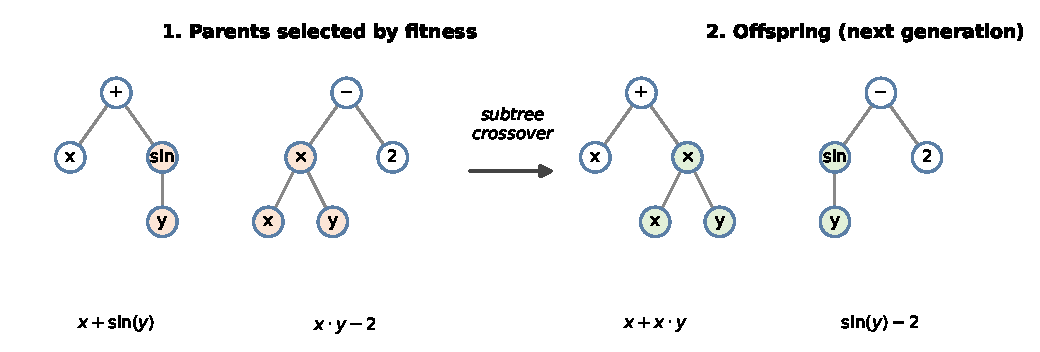
\includegraphics[width=0.95\linewidth]{figures/fig_genetic_tree.pdf}
    \caption[Key stages of Genetic Programming for SR]{Key stages of Genetic Programming for symbolic regression. Two parent trees are selected by fitness from the population; subtree crossover exchanges the highlighted segments, producing two offspring that enter the next generation. Figure inspired by \cite{Koza1992}.}
    \label{fig:genetic-tree}
\end{figure}

Selection is based on fitness: individuals with higher scores are copied and ``survive'' into the new generation. Genetic recombination occurs between two individuals that can vary in size and shape, and their offspring differ from both parents. The idea is that combining parts of two effective solutions may produce an even more effective one. The new population is evaluated, and the process repeats until a termination criterion is met \cite{Koza1992}. Figure~\ref{fig:genetic-tree} gives an overview of this classic process.

While effective in its search, GP has known drawbacks, including the risk of generating \textbf{overfit expressions} (which perform well on training data but poorly on new data), failure to recover the exact solution, and the absence of prior knowledge that could be transferred between problems \cite{Koza1992, dong2025RecentAdvances} --- each new task restarts the search from scratch.

\subsection{Neural Network-based Methods}

Artificial Neural Networks (ANNs), or simply Neural Networks (NNs), are computational models inspired by the structure and function of biological neurons. A neuron in an NN is a single computational unit: it takes a set of real numbers as inputs and produces a single output after performing a series of operations on them \cite{jm3_llm_book}. The primary operation is a weighted sum of the inputs plus a bias term:

\begin{equation}
    z = w \cdot x + b
    \label{eq:linear}
\end{equation}

where $z$ is the pre-activation output, $w$ the weight, $x$ the input, and $b$ the bias. The result $z$ is then passed through an activation function, which introduces non-linearity. A classical choice is the sigmoid function ($\sigma$), which maps $z$ to a value between 0 and 1:

\begin{equation}
    y = \sigma(z) =\frac{1}{1+ e^{-z}}
    \label{eq:sigma}
\end{equation}

Combining the two operations, the output of a single artificial neuron is:

\begin{equation}
    y = \sigma( w \cdot x + b) =\frac{1}{1+ \exp({-(w \cdot x + b)})}
    \label{eq:full_neuron}
\end{equation}

\begin{figure}[htbp]
    \centering
    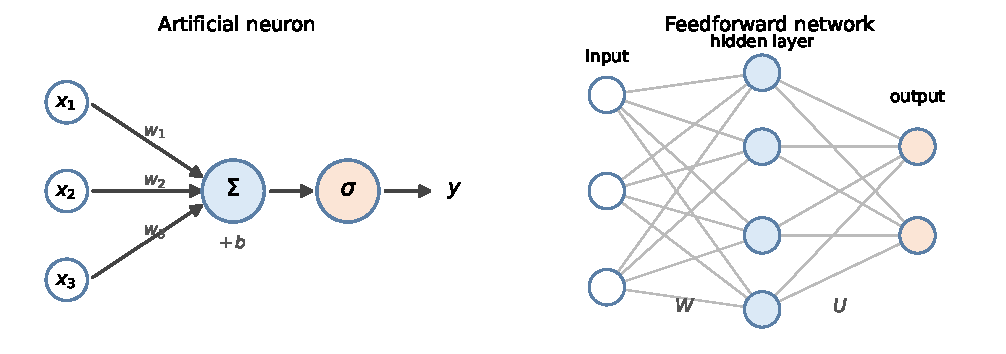
\includegraphics[width=0.9\linewidth]{figures/fig_neuron.pdf}
    \caption[Artificial neuron and feedforward network]{On the left, an artificial neuron: weighted inputs are summed with a bias and passed through an activation function $\sigma$ to produce the output $y$. On the right, a feedforward network: inputs connect to a hidden layer through weights $W$, whose outputs feed an output layer through weights $U$; information flows in one direction only. Inspired by \cite{jm3_llm_book}.}
    \label{fig:neuron}
\end{figure}

Neural networks are typically structured as collections of these units organized into interconnected layers. In the common \textit{feedforward} configuration, illustrated in Figure~\ref{fig:neuron}, units are arranged in layers without cyclic connections, and information flows unidirectionally: outputs of one layer are passed forward exclusively to the next \cite{jm3_llm_book}. The intermediate ``hidden layers'' transform the representation received from the preceding layer; each hidden unit has weights and a bias as parameters, and its computation follows the three steps above --- weighted sum, bias, activation \cite{jm3_llm_book}. The final, output layer converts the last hidden representation into the desired output format: a real number, a class decision, or a probability distribution (often via the softmax function) \cite{jm3_llm_book}.

NNs are used in supervised learning problems, where each observation $x$ comes with a correct output $y$ and the network produces a prediction $\hat{y}$. Training minimizes the distance between the two by adjusting the network parameters, using a loss function such as the \textbf{cross-entropy loss} for classification. The \textbf{backpropagation} algorithm computes the gradient of the loss with respect to every weight by applying the chain rule layer by layer; an optimizer such as \textbf{stochastic gradient descent} then updates the weights \cite{jm3_llm_book}.

Three hyperparameters recur throughout this work. An \textbf{epoch} is one complete pass through the training dataset; multiple epochs are usually needed for convergence. The \textbf{batch size} is the number of samples processed before each parameter update: smaller batches give noisier but more frequent updates, larger batches give stabler gradients at higher memory cost. The \textbf{learning rate} controls the step size of each update --- too high and the optimizer overshoots; too low and training crawls or stalls in local minima \cite{jm3_llm_book}. Tuning these values carefully turns out to be not merely a matter of efficiency but, as Chapter~\ref{ch:results} shows, a matter of experimental validity.

\section{Language Models}

A language model (LM) is a machine learning model that predicts the next word in a sequence based on probability. This deceptively simple objective supports a wide range of applications, including speech recognition, machine translation, and text generation.

\subsection{Overview of Language Models}

The idea that the probability of an event depends only on a limited number of preceding events is known as the Markov assumption. In the context of LMs, the goal is to predict the next token given the previous ones. A \textbf{token} can be a character, a subword unit, or a whole word. Subword tokenization (such as Byte Pair Encoding or WordPiece) is widely adopted \cite{jm3_llm_book}, primarily because it allows models to handle any text --- including rare or out-of-vocabulary words --- without the cost of representing every possible complete word.

Tokenization converts raw text into a sequence of standardized tokens mapped to unique numerical identifiers. These identifiers do not carry meaning by themselves; semantics is provided by the \textbf{embedding} process, which maps each token to a dense vector of real numbers \cite{jm3_llm_book}.

Traditional n-gram models compute the probability of a word from its frequency of occurrence after a fixed number of preceding words. While foundational, they suffer from limited context: only a short window of prior words can be considered, leading to data sparsity and an inability to capture long-range dependencies. Early feedforward neural language models shared this fixed-window limitation \cite{jm3_llm_book}.

Modern neural LMs are trained primarily through \textbf{self-supervision}: the model learns by predicting the next token in a large corpus of unlabeled text. This allows the network to discover useful representations of language --- including the embeddings themselves --- as part of training. The idea of learning rich contextual representations is central to the architectures discussed next \cite{jm3_llm_book}.

\subsection{Recurrent Neural Networks}

Recurrent Neural Networks (RNNs) are neural networks designed for sequential data such as audio or text \cite{Elman1990FindingSI}. In natural language, the order of words is essential to meaning. The term ``recurrent'' refers to the network repeating the same computation for each element of a sequence, with the output of one step feeding into the next --- giving the network a form of ``memory'' of what it has processed so far.

At each time step $t$, an RNN receives the current input $x_t$ (a word embedding) and a \textbf{hidden state} $h_{t-1}$ carrying information from previous steps; it produces an output $y_t$ and an updated hidden state $h_t$. Word embeddings are learned so that words appearing in similar contexts (e.g., \textit{friends} and \textit{family}) lie close together in the vector space, while unrelated words (e.g., \textit{car}) lie farther apart \cite{jm3_llm_book}.

RNNs struggle with long sequences. When trained with Backpropagation Through Time, gradients must propagate from the last step back to the first; the product of many gradient terms can shrink toward zero (\textbf{vanishing gradients}) or grow uncontrollably (\textbf{exploding gradients}), making convergence slow or unstable \cite{jm3_llm_book}. Successor architectures, notably Long Short-Term Memory (LSTM) networks \cite{Hochreiter1997LongSM} and Gated Recurrent Units (GRUs), mitigate these limitations and became the standard recurrent choices in NLP before the Transformer era \cite{jm3_llm_book}.

\subsection{Transformer Architecture}

The Transformer architecture was introduced to overcome fundamental limitations of recurrent models in sequence transduction tasks: their inherently sequential computation, which hinders parallelization, and their difficulty in capturing very long-range dependencies \cite{vaswani2017_attention_is_all}. The Transformer relies solely on attention mechanisms to draw global dependencies within sequences, allowing much greater parallelism and achieving state-of-the-art results on machine translation \cite{jm3_llm_book, vaswani2017_attention_is_all}.

The original Transformer follows an encoder--decoder design. The \textbf{encoder} maps an input sequence ($x_1, \ldots, x_n$) to a sequence of continuous representations; the \textbf{decoder} then generates the output sequence ($y_1, \ldots, y_m$) one token at a time, consuming previously generated tokens as additional input \cite{jm3_llm_book}. Both stacks consist of identical layers ($N=6$ in the original work). Each encoder layer has two sub-layers --- Multi-Head Self-Attention and a position-wise Feed-Forward Network (FFN) --- while decoder layers add a third sub-layer attending over the encoder output. All sub-layers produce outputs of a consistent dimension $d_{model}$ (512 in the original paper) \cite{vaswani2017_attention_is_all}.

The key component is \textbf{Multi-Head Self-Attention}. An attention function maps a query and a set of key--value pairs to an output. In self-attention, each token's embedding is linearly projected into three learned vectors: a \textbf{Query (Q)}, a \textbf{Key (K)}, and a \textbf{Value (V)} \cite{vaswani2017_attention_is_all}. The similarity between the Query of a token and the Keys of all tokens is computed via scaled dot products (division by $\sqrt{d_k}$ prevents large magnitudes from pushing the softmax into regions of tiny gradients); a softmax turns these similarities into attention weights, which produce a weighted sum of the Values \cite{jm3_llm_book, vaswani2017_attention_is_all}. Multi-Head Attention performs several such operations in parallel (e.g., $h=8$ heads with $d_k=d_v=d_{model}/h=64$), each with its own projections, letting the model attend to different representation subspaces simultaneously; the heads' outputs are concatenated and projected back to $d_{model}$ \cite{vaswani2017_attention_is_all}. In the decoder, a causal mask prevents positions from attending to subsequent positions, preserving the auto-regressive property.

Because the Transformer contains no recurrence or convolution, it cannot inherently encode token order. \textbf{Positional encodings} --- learned or fixed sinusoidal patterns --- are therefore added to the input embeddings \cite{jm3_llm_book, vaswani2017_attention_is_all}. Each FFN consists of two linear transformations with a ReLU activation in between, with an inner dimensionality $d_{ff}$ typically larger than $d_{model}$ (2048 for $d_{model}=512$) \cite{jm3_llm_book}.

A significant advantage of the architecture is its parallelism during training: attention for all tokens is computed simultaneously through matrix operations, greatly accelerating training compared to the sequential nature of RNNs. Its main cost is the quadratic complexity of attention with respect to sequence length. Nevertheless, the ability to capture long-range dependencies and the training efficiency established Transformers as the dominant architecture for modern large language models \cite{jm3_llm_book}.

\subsubsection{GPT-2}

Generative Pre-trained Transformer 2 (GPT-2) is a large-scale language model built upon the Transformer architecture. Unlike encoder--decoder variants, GPT-2 is a \textbf{decoder-only} Transformer, a design tailored for unidirectional (left-to-right) language generation \cite{radford2019language}: it predicts each token conditioned solely on the preceding sequence, enforced by causal masking in its self-attention layers. Architectural changes relative to the first GPT include moving layer normalization to the input of each sub-block, adding a final layer normalization after the last self-attention block, a depth-aware initialization scheme, a context window expanded from 512 to 1024 tokens, and a larger training batch size \cite{radford2019language}.

The family spans four sizes. The smallest model, with 117--124 million parameters, is comparable to the original GPT; intermediate versions have 345--355 million and 762--774 million parameters; and the largest, usually referred to simply as GPT-2, has 1.5 billion parameters \cite{jm3_llm_book, radford2019language}. In this work we use the three smaller sizes, referred to as Base, Medium, and Large.

GPT-2 was pre-trained by self-supervision on \textbf{WebText}, a corpus of over 8 million documents (40\,GB of text) curated by scraping outbound links from Reddit with at least 3 karma as a heuristic for human-filtered quality \cite{radford2019language}.\footnote{\textbf{Reddit} is a large social news aggregation and discussion website organized around user-submitted posts and links. \textbf{Karma} is a reputation score computed primarily from the net upvotes a user's contributions receive; higher karma indicates content valued by the community.} A key capability demonstrated by GPT-2 is zero-shot and few-shot learning: performing tasks such as reading comprehension, summarization, and translation without task-specific supervised training \cite{radford2019language}. On the other hand, it can produce factually inaccurate text (``hallucinations''), and its outputs are sensitive to the precise phrasing of the input prompt \cite{radford2019language} --- two behaviors that matter directly when the desired output is a syntactically strict mathematical expression.

\subsubsection{Fine-Tuning and Parameter-Efficient Adaptation}
\label{sec:bg_finetuning}

Pre-training endows an LM with general linguistic competence, but specific tasks usually require \textbf{fine-tuning}: continuing training on a smaller, task-specific corpus so the model's distribution shifts toward the target domain \cite{jm3_llm_book}. Full fine-tuning updates all parameters, which for models with hundreds of millions of weights is memory- and compute-intensive and produces a full model copy per task.

Parameter-Efficient Fine-Tuning (PEFT) techniques address this cost by updating only a small set of additional parameters. The method used in this work, \textbf{Low-Rank Adaptation (LoRA)} \cite{hu2021lora}, freezes the pre-trained weights and injects trainable low-rank matrices into selected layers: a weight update $\Delta W \in \mathbb{R}^{d \times k}$ is factorized as $\Delta W = BA$ with $B \in \mathbb{R}^{d \times r}$, $A \in \mathbb{R}^{r \times k}$, and rank $r \ll \min(d, k)$. Only $A$ and $B$ are trained --- typically well under 1\% of the original parameter count --- and after training the product $BA$ can be merged back into the frozen weights, leaving inference cost unchanged. The rank $r$ and a scaling factor $\alpha$ control the capacity of the adaptation.

\section{Deep Reinforcement Learning}

Deep Reinforcement Learning (DRL) combines the principles of Reinforcement Learning (RL) with deep neural networks, enabling agents to learn directly from high-dimensional inputs such as images or raw text, without manual feature engineering. A seminal work is the Deep Q-Network (DQN) \cite{Mnih2015HumanlevelCT}, which reached human-level control on Atari games by training a deep network to estimate action values directly from pixels --- a demonstration that opened the field to problems previously intractable for classical RL.

\subsection{Reinforcement Learning}

Reinforcement Learning is a computational approach to goal-directed learning through interaction \cite{Sutton2018ReinforcementL}. Unlike supervised learning, which relies on labeled examples, or unsupervised learning, which seeks hidden structure, RL agents learn by acting in an environment and receiving a numerical reward signal to be maximized over time. The agent is not told which actions to take; it must discover effective behavior by trial and error \cite{Sutton2018ReinforcementL}.

The fundamental elements of an RL system are \cite{Sutton2018ReinforcementL}:
\begin{itemize}
    \item \textbf{Agent}: the learner and decision-maker.
    \item \textbf{Environment}: everything outside the agent, with which it interacts.
    \item \textbf{State ($S$)}: a representation of the current situation perceived by the agent.
    \item \textbf{Action ($A$)}: a choice made by the agent that can influence the environment.
    \item \textbf{Reward ($R$)}: a scalar feedback indicating the immediate desirability of the agent's action; the agent's objective is to maximize cumulative reward.
    \item \textbf{Policy ($\pi$)}: the agent's behavior --- a (possibly stochastic) mapping from states to actions.
    \item \textbf{Value function ($V$ or $Q$)}: the long-run counterpart of the reward --- the total reward an agent can expect starting from a state (or state--action pair).
\end{itemize}

A central challenge is the \textbf{exploration--exploitation dilemma}: the agent must balance exploiting actions known to be good against exploring new actions that might be better \cite{Sutton2018ReinforcementL}. This dilemma, as we will see, is not an abstract concern --- it is the axis along which the algorithms compared in this work differ most.

\subsection{Policy Gradient Methods}

Policy gradient methods directly optimize the agent's policy without necessarily relying on a value function to select actions \cite{Sutton2018ReinforcementL}. They parameterize the policy by $\theta$ and perform gradient ascent on the performance objective $J(\theta)$, estimating the direction in parameter space that most rapidly improves performance.

A foundational algorithm is REINFORCE \cite{Williams1992Simple}, a statistical gradient-following method that adjusts the policy parameters along the gradient of expected reinforcement:
\begin{equation}
    \nabla_\theta J(\theta) = \mathbb{E}\left[ \nabla_\theta \log \pi_\theta(a|s) \cdot (R - b) \right]
\end{equation}
where $b$ is a baseline used for variance reduction. While theoretically sound, vanilla policy gradients often suffer from poor data efficiency and robustness \cite{Schulman2017ProximalPO}. Trust Region Policy Optimization (TRPO) \cite{Schulman2015TrustRP} improved stability by constraining the size of each policy update: it maximizes a surrogate objective subject to a bound on the Kullback--Leibler (KL) divergence between the new and old policies.

\subsection{Actor-Critic Methods}

A complementary way to reduce the variance of policy gradients is to learn a value function that guides the policy updates, giving rise to \textbf{Actor--Critic methods}. These combine a policy-based component --- the \textbf{actor}, which decides which action to take --- with a value-based component --- the \textbf{critic}, which evaluates the actor's choices. Modern actor--critic methods rely on the \textbf{advantage function},
\begin{equation}
    A^\pi(s, a) = Q^\pi(s, a) - V^\pi(s),
\end{equation}
which measures how much better action $a$ is than the policy's average behavior in state $s$. Increasing the probability of positive-advantage actions is the core of algorithms such as Asynchronous Advantage Actor--Critic (A3C) \cite{mnih2016asynchronous}.

\subsection{Proximal Policy Optimization (PPO)}

Proximal Policy Optimization (PPO) is a family of policy gradient methods that balances sample complexity, implementation simplicity, and performance \cite{Schulman2017ProximalPO}. PPO pursues the reliability of TRPO while requiring only first-order optimization. Its core innovation is the \textit{clipped surrogate objective}:
\begin{equation}
 L^{CLIP}(\theta) = \hat{\mathbb{E}}_{t}\left[\min\left(r_t(\theta)\hat{A}_t,\; \text{clip}(r_t(\theta), 1-\epsilon, 1+\epsilon)\hat{A}_t\right)\right]
 \label{eq:ppo_clip}
\end{equation}
where $r_t(\theta) = \frac{\pi_{\theta}(a_t|s_t)}{\pi_{\theta_{old}}(a_t|s_t)}$ is the probability ratio between the new and old policies and $\hat{A}_t$ is an advantage estimate. The $\min$ combined with the clip keeps updates within a ``proximal'' region around the old policy, penalizing probability ratios outside $[1-\epsilon, 1+\epsilon]$ (e.g., $\epsilon = 0.2$) and yielding a pessimistic lower bound on policy improvement. PPO alternates between collecting data with the current policy and performing several epochs of stochastic gradient ascent on the collected batch, typically combining the clipped objective with a value-function loss and an entropy bonus for exploration, while monitoring the KL divergence between successive policies \cite{Schulman2017ProximalPO}. Its robustness across domains made PPO the default algorithm for fine-tuning language models with reinforcement learning \cite{ouyang_training_2022}.

\subsection{Group Relative Policy Optimization (GRPO)}
\label{sec:bg_grpo}

Group Relative Policy Optimization (GRPO) is a more recent policy-gradient variant, introduced for mathematical-reasoning LLMs \cite{shao2024deepseekmath} and popularized by the DeepSeek-R1 training pipeline \cite{deepseek_r1_2025}. GRPO dispenses with the learned critic: for each prompt, the policy samples a \emph{group} of $G$ responses, and the advantage of each response is computed \emph{relative to the group},
\begin{equation}
    \hat{A}_i = \frac{r_i - \mathrm{mean}(r_1, \ldots, r_G)}{\mathrm{std}(r_1, \ldots, r_G)},
    \label{eq:grpo_adv}
\end{equation}
optionally using ranks instead of raw rewards for additional robustness to reward scale. The normalized advantages then enter a PPO-style clipped objective, usually with an explicit KL penalty toward a reference policy. Removing the value network halves the memory footprint and eliminates a source of estimation error, which is particularly attractive when the reward is computed at the sequence level --- exactly the case in symbolic regression, where a complete expression receives a single score. The group normalization, however, has a flip side that Chapter~\ref{ch:results} examines empirically: when most responses in a group receive similar rewards, the normalized advantages shrink and the selective pressure of the update weakens.

\subsection{Reinforcement Learning for Language Models}
\label{sec:bg_rl_llm}

Fine-tuning language models with RL follows a common recipe, established at scale by InstructGPT \cite{ouyang_training_2022}: the LM is treated as a policy $\pi_\theta$ whose ``action'' is the generation of a token sequence; a scalar reward scores each complete generation; and a policy-gradient algorithm (typically PPO) updates the model to increase expected reward, with a KL term keeping the policy close to its supervised initialization. In this framing, generation is an episodic RL problem with a single terminal reward --- there is no intermediate feedback while the sequence is being written.

A much simpler alternative requires no gradient updates at all: \textbf{Best-of-N (BoN) sampling}, in which $N$ candidate generations are drawn from the frozen model and the best-scoring one is returned \cite{stiennon2020learning}. BoN is a strong and frequently underestimated baseline: given a large enough $N$, it exposes everything the underlying model can produce. For this reason, any claim that RL ``improves'' a generator is only meaningful against a BoN baseline given the same sampling budget --- a principle that shaped the experimental design of this work.

Between pure sampling and pure RL lies a family of techniques that \emph{retain} the best discoveries and reuse them as training signal. In symbolic regression, Priority Queue Training \cite{petersen2020deep} maintains a queue of the highest-reward expressions and mixes them into the training batches, anchoring the policy to known good solutions while it continues to explore. The \textbf{elite buffer} used in this work belongs to this family: a bounded, deduplicated memory of the top-$K$ expressions found so far, from which a fraction of each training batch is re-sampled. The interaction between this retention mechanism and the exploration profile of the update algorithm (PPO vs.\ GRPO) is the central experimental question of the thesis.

\section{Related Work}

This review examines the trajectory of the field of symbolic regression, first covering the foundational techniques in GP and then detailing the recent advances driven by Transformers and large language models.

\subsection{Genetic Programming as a Classical Approach for Symbolic Regression}

The process of developing models to understand natural phenomena is a fundamental aspect of the scientific method. As pointed out by Dong et al. \cite{dong2025RecentAdvances} and Cranmer \cite{cranmer2023interpretable}, the trial-and-error process of finding a symbolic model from observations was crucial for Kepler's laws of planetary motion and Newton's law of universal gravitation. The work that introduced GP for SR was Koza's \cite{Koza1992}, which details the foundational paradigm where populations of computer programs are ``genetically bred'' through natural selection and crossover to solve problems including symbolic regression, and introduces automatically defined functions for hierarchical problem decomposition. In GP, the individuals are the programs themselves, commonly represented as rooted, point-labeled trees corresponding to LISP S-expressions; genetic operators such as subtree crossover manipulate these tree structures directly.

In contrast, Grammatical Evolution (GE) \cite{oneill_grammatical_2003} evolves simple binary strings that are translated into syntactically correct programs by a formal (Backus--Naur Form) grammar, separating the search space (genotype) from the solution space (phenotype) and avoiding the syntactically invalid programs that plague naive GP. As GP systems grew in complexity, premature convergence to local optima became a critical concern. Schmidt and Lipson \cite{schmidt2011age} proposed Age-Fitness Pareto Optimization, which treats the genotypic age of an individual as a second optimization objective alongside fitness; by allowing younger, less-fit individuals to survive and mature, it preserves exploration and reduces the risk of a single high-fitness lineage dominating the population.

La Cava et al. \cite{cava_epsilon-lexicase_2016} point out that selecting individuals based only on an aggregate test score is problematic for SR. Their $\epsilon$-lexicase selection admits individuals whose error is within $\epsilon$ of the best on individual data cases, with mechanisms to adapt $\epsilon$ automatically; this favors specialists that excel on different subsets of the data, increasing diversity and leading to more accurate final models.

Traditional GP operators manipulate syntax blindly: a small change to a tree can cause a drastic, unpredictable change in its output --- a property known as low locality \cite{uy_semantically-based_2011}. Semantic GP designs operators that induce more controlled changes in behavior. An early approach is Semantic Similarity-based Crossover \cite{uy_semantically-based_2011}, which defines the semantics of a subtree as its vector of outputs on sample data points and only swaps subtrees that are semantically similar but not identical, improving search locality. Moraglio et al. \cite{moraglio2012gsgp}, with Geometric Semantic GP, formalized search in semantic space with exact geometric operators guaranteeing that offspring lie on the semantic segment between their parents, transforming the fitness landscape into an easily searchable cone --- at the cost of expression growth that requires computer algebra systems to simplify.

Building on these ideas, Virgolin et al. \cite{virgolin_improving_2019} enhance Semantic Backpropagation-based GP by integrating Linear Scaling both synergistically with semantic backpropagation and within the library search process \cite{virgolin2019linear}, significantly reducing error compared to traditional operators. Kommenda et al. \cite{kommenda2020parameter} explore nonlinear least squares (Levenberg--Marquardt) for parameter identification within GP-based SR, showing that local constant optimization substantially improves accuracy and generalization for differentiable models. GP-GOMEA \cite{virgolin_improving_2019} learns a statistical model of interdependencies between tree nodes (a linkage model) and uses it to guide a Gene-pool Optimal Mixing operator that recombines promising sub-components. Generalized Symbolic Regression \cite{tohme2022gsr} reformulates the problem itself, searching for models of the form $g(y) = f(x)$ rather than $y = f(x)$: a GP evolves basis functions for inputs and outputs, and a Lasso regression finds an optimal sparse linear combination, often uncovering simpler solutions (e.g., $\ln(y) = \cos(x)$ instead of $y = e^{\cos(x)}$).

The increasing sophistication of hybrid methods has driven the development of software frameworks that make SR practical for scientific applications. PySR provides a user-friendly Python interface to a high-performance Julia backend implementing an evolve--simplify--optimize loop; Operon is a C++ framework using a cache-friendly linear tree encoding and a scalable concurrency model; Bingo \cite{randall_bingo_2022} offers a modular Python architecture for custom hybrid workflows. Together, these frameworks illustrate a trend toward making advanced SR methods more efficient and accessible.

As summarized by Dong et al. \cite{dong2025RecentAdvances}, GP remains a powerful and interpretable approach, with adaptability stemming from diverse chromosome representations and numerous refinements to its operators. However, the vast search space makes GP prone to overfitting; performance is sensitive to hyperparameters; the method struggles with high-dimensional data (``curse of dimensionality''); it risks entrapment in local optima; and it is computationally intensive, often requiring parallel or distributed computing at scale. Crucially for the present work, classical GP also starts every problem from zero --- it has no mechanism to accumulate knowledge across tasks, which is precisely the gap that pre-trained models address.

\subsection{Language Models for Expression Finding}
\label{sec:related_lm}

The advent of deep learning introduced a new paradigm for SR. By pre-training on large, synthetically generated datasets, sequence models learn implicit priors about the structure of mathematical expressions, reframing SR from a pure search problem into one where discovery is guided by learned knowledge.

A significant step was Deep Symbolic Regression (DSR) \cite{petersen2020deep}, which trains an RNN with a risk-seeking policy gradient that rewards the single best expression found rather than average performance --- a foundational technique for the field and, through its Priority Queue Training variant, a direct ancestor of the elite buffer studied here. The same group extended the idea to control problems with Deep Symbolic Policy \cite{landajuela_discovering_2021}. DSR outperformed contemporaneous baselines, though it was slower than GP without early stopping and failed on certain complex structures.

The Transformer architecture \cite{vaswani2017_attention_is_all} brought sequence-to-sequence pre-training to SR. Biggio et al. \cite{biggio_neural_2021} proposed NeSymReS, the first method to leverage large-scale pre-training: standard Transformer encoder--decoder blocks trained on millions of synthetic equations to predict expression ``skeletons'', treating SR as a translation problem. Similarly, SymbolicGPT \cite{valipour_symbolicgpt_2021} frames SR as a captioning task in which a point-cloud encoder and a GPT-style decoder translate data into an equation skeleton. Both predict only the structure and fit constants in a post-processing optimization step. Kamienny et al. \cite{kamienny2022end} later showed that Transformers can predict complete expressions, constants included, end to end. In the same period, uDSR \cite{landajuela_unified_2022} unified DSR, AI Feynman \cite{udrescu_ai_2019, ai_feyman2}, genetic programming, and large-scale pre-training in a modular framework, demonstrating the power of hybridization.

Later works refined training and inference. TPSR \cite{shojaee_transformer-based_2023} uses Monte Carlo Tree Search to guide the decoding of a pre-trained transformer, optimizing non-differentiable equation-level objectives such as accuracy and complexity. Deep Generative Symbolic Regression (DGSR) \cite{holt_deep_2023} improves computational efficiency through a pre-training and refinement strategy whose end-to-end NMSE loss allows gradient-based fine-tuning on a new problem at inference time. New training objectives also emerged: T-JSL \cite{li_transformer-based_2023} uses a supervised contrastive loss to distinguish expressions sharing a skeleton but differing in constants, and ODEFormer \cite{dascoli_odeformer_2023} infers symbolic ordinary differential equations directly from noisy, sparse trajectory data.

The most recent wave relies on general-purpose LLMs rather than SR-specific models trained from scratch. LLM-SR \cite{shojaee_llm-sr_2024} and the FunSearch line of work \cite{ellenberg_generative_2025} use an LLM as an intelligent mutation and crossover operator within an evolutionary loop, generating program code for candidate equations. LASR \cite{grayeli2024symbolicregressionlearnedconcept} performs a two-stage evolution over natural-language concepts and programmatic hypotheses, with the LLM distilling recurring ideas from the best candidates into a growing concept library. In-Context Symbolic Regression \cite{merler_-context_2024} uses an iterative loop in which Llama~3 \cite{grattafiori2024llama3herdmodels} is prompted with high-performing equations from previous rounds to propose better ones, requiring no task-specific training. FormulaGPT \cite{li_generative_2024} applies ``algorithmic distillation'', training a transformer on the search histories of RL-based SR algorithms to internalize their search policies. SR-GPT \cite{li_discovering_2024} couples a GPT model with MCTS in a self-play loop where search data continually refines the model.

A newer trend explores multimodality and interactivity. SNIP \cite{meidani_snip_2023} and MMSR \cite{li_mmsr_2024} treat SR as an intrinsically multimodal task, using contrastive learning to align latent representations of numeric data and symbolic expressions as if they were two languages. Sym-Q \cite{tian_interactive_2025} is an offline-RL framework whose co-design mechanism lets a domain expert provide partial equations to guide the search interactively.

\vspace{0.5em}
Table~\ref{tab:related_work} summarizes the main works discussed in this section.

\begin{small}
\begin{longtable}{>{\raggedright}p{0.20\linewidth} >{\centering}p{0.07\linewidth} >{\raggedright}p{0.47\linewidth} >{\centering\arraybackslash}p{0.14\linewidth}}
\caption{Overview of neural and LLM-based symbolic regression methods.}
\label{tab:related_work}\\
\toprule
\textbf{Work} & \textbf{Year} & \textbf{Model/Method} & \textbf{Parameters} \\
\midrule
\endfirsthead

\multicolumn{4}{c}%
{{\bfseries Table \thetable\ continued from previous page}} \\
\toprule
\textbf{Work} & \textbf{Year} & \textbf{Model/Method} & \textbf{Parameters} \\
\midrule
\endhead

\bottomrule
\endfoot

\textbf{DSR} \cite{petersen2020deep} & 2020 & RNN + risk-seeking RL & -- \\
\addlinespace
\textbf{NeSymReS} \cite{biggio_neural_2021} & 2021 & Encoder--Decoder Transformer & 24M \\
\addlinespace
\textbf{SymbolicGPT} \cite{valipour_symbolicgpt_2021} & 2021 & Encoder--Decoder (T-net + GPT) & -- \\
\addlinespace
\textbf{uDSR} \cite{landajuela_unified_2022} & 2022 & Hybrid (Transformer, RNN, GP, RL) & -- \\
\addlinespace
\textbf{E2E} \cite{kamienny2022end} & 2022 & Encoder--Decoder Transformer & 86M \\
\addlinespace
\textbf{DGSR} \cite{holt_deep_2023} & 2023 & Encoder--Decoder Transformer + RL/GP & -- \\
\addlinespace
\textbf{TPSR} \cite{shojaee_transformer-based_2023} & 2023 & Pre-trained Transformer + MCTS & -- \\
\addlinespace
\textbf{T-JSL} \cite{li_transformer-based_2023} & 2023 & Encoder--Decoder (PointMLP + GPT) & -- \\
\addlinespace
\textbf{ODEFormer} \cite{dascoli_odeformer_2023} & 2023 & Encoder--Decoder Transformer & 86M \\
\addlinespace
\textbf{SNIP} \cite{meidani_snip_2023} & 2023 & Multimodal Encoder--Decoder & -- \\
\addlinespace
\textbf{FormulaGPT} \cite{li_generative_2024} & 2024 & Transformer + algorithmic distillation & -- \\
\addlinespace
\textbf{MMSR} \cite{li_mmsr_2024} & 2024 & Multimodal Encoder--Decoder & -- \\
\addlinespace
\textbf{LLM-SR} \cite{shojaee_llm-sr_2024} & 2024 & LLM + evolutionary search & -- \\
\addlinespace
\textbf{LASR} \cite{grayeli2024symbolicregressionlearnedconcept} & 2024 & LLM + genetic programming & -- \\
\addlinespace
\textbf{ICSR} \cite{merler_-context_2024} & 2024 & LLM (Llama 3) + iterative prompting & 8B \\
\addlinespace
\textbf{SR-GPT} \cite{li_discovering_2024} & 2024 & GPT + MCTS self-play & -- \\
\addlinespace
\textbf{FunSearch line} \cite{ellenberg_generative_2025} & 2025 & LLM + genetic algorithm & -- \\
\addlinespace
\textbf{Sym-Q} \cite{tian_interactive_2025} & 2025 & Offline RL Q-network & -- \\
\addlinespace
\textbf{Seriguela (ours)} & 2026 & SFT GPT-2 + RL (PPO/GRPO $\pm$ elite buffer) & 124M \\
\end{longtable}
\end{small}

\subsection{Positioning of This Work}
\label{sec:positioning}

Within this landscape, Seriguela occupies a deliberate middle ground. Unlike NeSymReS, E2E, or DGSR, we do not train an SR-specific architecture from scratch: we start from a general-purpose, publicly available LM (GPT-2) and adapt it with parameter-efficient fine-tuning, testing how far the ``language of mathematics'' can be grafted onto a model pre-trained on natural text. Unlike LLM-SR, LASR, or ICSR, we do not rely on frozen billion-parameter models steered by prompting: our policy is small (124M parameters), fully under our control, and \emph{updated} by on-line reinforcement learning. And unlike DSR --- the closest conceptual relative --- our generator is a pre-trained Transformer rather than an RNN trained from scratch, and our policy updates use the modern PPO/GRPO family developed for LLM alignment rather than a risk-seeking vanilla policy gradient.

This position lets the thesis ask a question the surveyed works leave open: \emph{given} a fixed pre-trained expression generator, which reinforcement-learning recipe extracts the most from it --- and why? The controlled five-arm comparison (Best-of-N, PPO, GRPO, each $\pm$ elite buffer, under a uniform reward and identical budget) and the exploration--retention analysis it supports are, to our knowledge, novel in the SR literature.

\chapter{Materials and Methods}
\label{ch:methods}

This chapter details the methodology of the Seriguela pipeline: the data engineering process for generating, cleaning, and formatting the mathematical-expression corpus; the supervised fine-tuning of the language models; the reinforcement learning framework for expression discovery, including the five algorithmic arms compared in this work; the benchmark suites and evaluation protocol; the phased experimental design; and the implementation and hardware environment.

\section{Overview of the Proposed Seriguela Pipeline}

\begin{figure}[htbp]
    \centering
    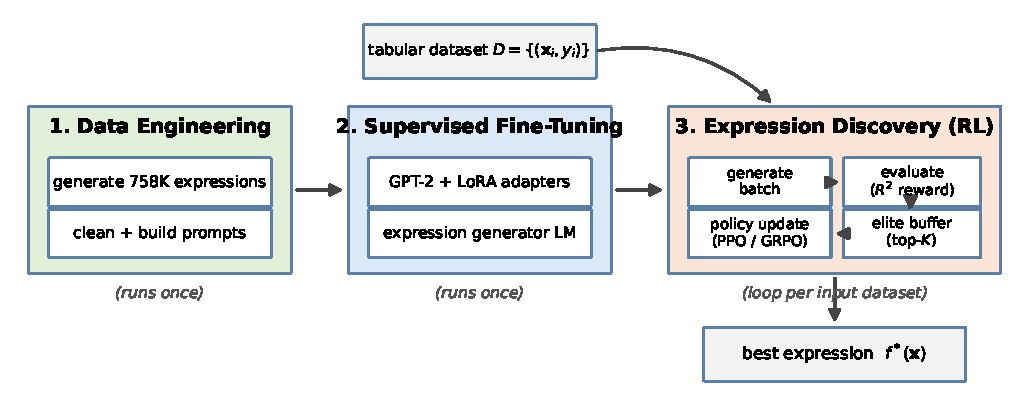
\includegraphics[width=0.98\linewidth]{figures/fig_overview.pdf}
    \caption[End-to-end overview of the Seriguela pipeline]{End-to-end overview of the Seriguela pipeline. Stages 1 and 2 run once and produce a reusable expression-generator model; stage 3 runs per input dataset, optimizing the generator toward the expression that best fits the data.}
    \label{fig:pipeline}
\end{figure}

As illustrated in Figure~\ref{fig:pipeline}, our approach implements a three-stage methodology for symbolic regression:

\begin{enumerate}
    \item \textbf{Data Engineering}: a large corpus of mathematical expressions is generated, validated to remove malformed samples, and formatted into structured training prompts.
    \item \textbf{Supervised Fine-Tuning (SFT)}: a pre-trained language model is specialized on this corpus, turning it into a domain-specific expression generator.
    \item \textbf{Expression Discovery}: the fine-tuned model is optimized with reinforcement learning against a specific tabular dataset, exploring and refining candidate expressions until one fits the data.
\end{enumerate}

The first two stages are executed only once; their cost is amortized over every subsequent problem. Stage 3 restarts for each new input dataset, always from the same SFT checkpoint.

\section{Dataset Engineering}

\begin{figure}[htbp]
    \centering
    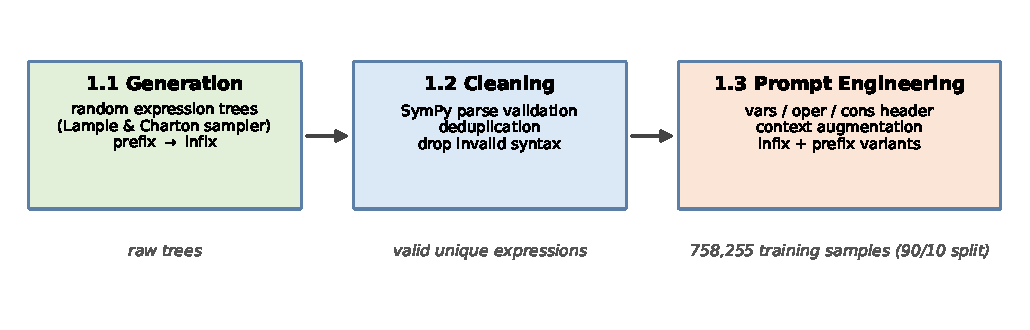
\includegraphics[width=0.98\linewidth]{figures/fig_data_engineering.pdf}
    \caption[Data engineering pipeline]{Data engineering pipeline of the expression corpus: (1.1) random generation of expression trees, (1.2) validation and deduplication, and (1.3) prompt construction.}
    \label{fig:DataEngineering}
\end{figure}

Large language models such as GPT-2 are pre-trained on vast amounts of natural language. Their core objective --- predicting the next most probable token --- is not inherently suited to the syntactically precise, computable language of mathematics. When prompted to produce an equation, a base GPT-2 model typically answers with descriptive text, incorrect formats, or syntactically invalid expressions, as illustrated in Table~\ref{tab:gpt2-comparison}.

To address this limitation, the model is specialized through supervised fine-tuning on a dedicated corpus of mathematical expressions. The data engineering pipeline that builds this corpus consists of three stages --- generation, cleaning, and prompt engineering --- outlined in Figure~\ref{fig:DataEngineering}.

\subsection{Dataset Generation}

\begin{table}[htbp]
    \centering
    \caption{Equation generation configuration parameters.}
    \label{tab:eq_config}
    \begin{tabular}{p{3cm}p{5.2cm}p{4.2cm}}
    \toprule
    \textbf{Parameter} & \textbf{Value} & \textbf{Description} \\
    \midrule
    \texttt{max\_len} & 20 & Maximum token length per equation \\
    \addlinespace
    \texttt{operators} &
    \texttt{add:10, mul:10, sub:5, div:5, sqrt:4, pow2:4, exp:4, sin:4, cos:4, tan:4, asin:2} &
    Operator sampling weights \\
    \addlinespace
    \texttt{max\_ops} & 5 & Maximum operations per equation \\
    \addlinespace
    \texttt{variables} & \texttt{x\_1, \ldots, x\_10} & Base variables (extensible via the \texttt{x\_n} convention) \\
    \bottomrule
    \end{tabular}
\end{table}

The first step was to generate a large volume of diverse mathematical expressions. Expressions are treated as tree structures in which internal nodes are operators (e.g., $+$, $\sin$, $\times$) and leaves are operands --- variables (e.g., $x_1, x_2$) or constants.

To sample these trees without biasing toward overly simple or overly deep structures, we adopted the algorithm proposed by Lample and Charton \cite{lample2019deep}, which gives different tree shapes a near-uniform probability of being generated. The algorithm handles internal nodes with one child (unary operators such as $\sin$) and two children (binary operators such as $+$). Expressions were first created in prefix notation and then converted to the more common infix format. The generation parameters are listed in Table~\ref{tab:eq_config}.

After cleaning and augmentation, the final corpus contains \textbf{758{,}255 expressions}, split into 682{,}429 training samples (90\%) and 75{,}826 validation samples (10\%). The dataset is publicly available on HuggingFace as \texttt{augustocsc/sintetico\_natural\_prefix\_682k}. Table~\ref{tab:dataset_stats} summarizes its statistics and the representation formats available per expression, and Table~\ref{tab:dataset_examples} shows concrete examples.

\begin{table}[htbp]
    \centering
    \caption{Final dataset statistics and available columns.}
    \label{tab:dataset_stats}
    \begin{tabular}{ll}
    \toprule
    \textbf{Statistic} & \textbf{Value} \\
    \midrule
    Total expressions & 758{,}255 \\
    Training split & 682{,}429 (90\%) \\
    Validation split & 75{,}826 (10\%) \\
    File format & Parquet (143 MB) \\
    \midrule
    \textbf{Column} & \textbf{Description} \\
    \midrule
    \texttt{infix\_expr\_n} & Infix notation (natural variables) \\
    \texttt{prefix\_expr\_n} & Prefix notation (natural variables) \\
    \texttt{i\_prompt\_n} & Complete infix prompt for training \\
    \texttt{p\_prompt\_n\_converted} & Complete prefix prompt for training \\
    \texttt{skeleton} & Expression template with variable wildcards \\
    \bottomrule
    \end{tabular}
\end{table}

\begin{table}[htbp]
    \centering
    \caption{Example expressions from the dataset in different formats.}
    \label{tab:dataset_examples}
    \begin{tabular}{p{2.5cm}p{10cm}}
    \toprule
    \textbf{Format} & \textbf{Example} \\
    \midrule
    Infix & \texttt{x\_1*x\_2 + exp(x\_2)} \\
    Prefix & \texttt{+ * x\_1 x\_2 exp x\_2} \\
    Skeleton & \texttt{V*V + exp(V)} \\
    \midrule
    Infix & \texttt{cos(x\_1 + C*x\_2)/sin(C*(C*x\_1 + C)**2)} \\
    Prefix & \texttt{/ cos + x\_1 * C x\_2 sin * C ** + * C x\_1 C C} \\
    Skeleton & \texttt{cos(V + C*V)/sin(C*(C*V + C)**C)} \\
    \bottomrule
    \end{tabular}
\end{table}

The corpus covers a comprehensive set of operators, summarized in Table~\ref{tab:operators}: basic arithmetic, trigonometric functions, and transcendental operations. Variables follow the naming convention \texttt{x\_1}, \texttt{x\_2}, \ldots, \texttt{x\_10}, allowing expressions with up to 10 input features, and constants are represented by the placeholder token \texttt{C}, whose treatment during discovery is discussed in Section~\ref{sec:c_protocol}.

\begin{table}[htbp]
    \centering
    \caption{Mathematical operators available in the dataset.}
    \label{tab:operators}
    \begin{tabular}{lll}
    \toprule
    \textbf{Category} & \textbf{Operators} & \textbf{Arity} \\
    \midrule
    Arithmetic & $+$, $-$, $\times$, $\div$, \texttt{**} (power) & Binary \\
    Trigonometric & $\sin$, $\cos$, $\tan$, $\arcsin$ & Unary \\
    Transcendental & $\exp$, $\log$ & Unary \\
    Other & $\sqrt{\cdot}$, $|\cdot|$ (abs) & Unary \\
    \bottomrule
    \end{tabular}
\end{table}

\begin{table}[htbp]
    \centering
    \caption{Comparison of the GPT-2 model's output before and after fine-tuning, demonstrating its improved ability to generate syntactically correct expressions.}
    \label{tab:gpt2-comparison}
    \ttfamily
    \begin{tabularx}{\textwidth}{ >{\RaggedRight}X >{\RaggedRight}X }
    \toprule
    \multicolumn{2}{c}{\textbf{Base Model}} \\
    \midrule
    \textbf{Prompt} & \textbf{Result} \\
    \midrule
    Generate a mathematical expression that represents the kinetic energy of an object with mass m and velocity v.
    &
    For example, if you want to calculate the kinetic energy of a baseball, you can use the following formula: $K=nx$ \\
    \addlinespace
    Write a trigonometric expression involving sine and cosine that simplifies to 1.
    &
    Write a trigonometric expression involving sin and cosine that simplifies to 1. \\
    \addlinespace
    Instruction: Generate a mathematical expression using variables [x\_1, x\_2, x\_3, x\_4], operands [+, -, *, exp], and [C] as a constant. Expression:
    &
    $x_1 = -(x_2 \cdot x_3) + (x_4 \cdot \exp)$ The expression above is a mathematical expression. \\
    \midrule[1pt]
    \multicolumn{2}{c}{\textbf{After Fine-Tuning}} \\
    \midrule
    vars: x\_1, \ldots, x\_9 \newline oper: *, **, +, -, abs, asin, cos, exp, log, sin, sqrt, tan \newline cons: C \newline expr:
    &
    $x_7 + \exp(C \cdot x_2^C) + C$ \\
    \bottomrule
    \end{tabularx}
\end{table}

\subsection{Data Cleaning}

To ensure the corpus's integrity, every expression was validated with a SymPy \cite{sympy} parser, which flags issues such as unbalanced parentheses or dangling operators. Duplicate expressions were removed to maintain uniqueness.

\subsection{Prompt Engineering}
\label{sec:prompt_engineering}

After generation and cleaning, the corpus was still a plain list of valid expressions --- unsuitable for fine-tuning for two reasons. First, bare expressions provide no \emph{guiding structure}: at inference time there would be no contextual prompt through which to steer generation. Second, the generator produces expressions with limited variable diversity (often five or fewer), and nothing teaches the model to cope with context it does not need.

A prompt engineering phase therefore transformed each raw expression into a structured training sample --- human-readable, token-efficient, and explicit about the elements available for generation:

\begin{verbatim}
vars: x_1, x_2, x_3, x_4, x_5, x_6, x_7, x_8, x_9
oper: *, **, +, -, abs, asin, cos, exp, log, sin, sqrt, tan
cons: C
expr: x_7 + exp(C*x_2**C) + C
\end{verbatim}

To enhance robustness, the \texttt{vars:} and \texttt{oper:} lists were intentionally over-provisioned: for each training sample, a random number of additional variables and operators --- beyond those strictly required by the target expression --- were included. This teaches the model to use only a \emph{subset} of the offered elements, mirroring real scenarios where not every feature is relevant. Finally, both the \textbf{infix} (standard) and \textbf{prefix} (Polish) representations were retained, allowing the notation format itself to be studied as a factor.

\section{Supervised Fine-Tuning}
\label{sec:sft_setup}

With the structured corpus prepared, the next stage teaches the pre-trained model to generate syntactically correct, well-formed expressions. For input processing, the original GPT-2 tokenizer was employed without modification, as its vocabulary adequately covers the mathematical symbols and variables in our data. A useful property of this tokenizer is its fine granularity: words like \texttt{asin} decompose into sub-tokens (\texttt{as}, \texttt{in}) and variables like \texttt{x\_1} into (\texttt{x}, \texttt{\_}, \texttt{1}). This sub-word tokenization, illustrated in Figure~\ref{fig:tokenization}, lets the model generalize to variables never seen during training, such as \texttt{x\_99}.

\begin{figure}[htbp]
    \centering
    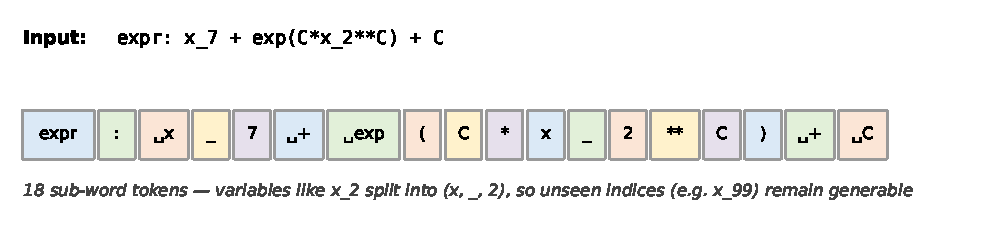
\includegraphics[width=0.95\textwidth]{figures/fig_tokenization.pdf}
    \caption[GPT-2 tokenization of a sample prompt]{GPT-2 tokenization of a sample prompt line. The marker \texttt{␣} denotes a leading space absorbed into the token. Because variables decompose into sub-tokens, unseen indices remain generable.}
    \label{fig:tokenization}
\end{figure}

Fine-tuning used the HuggingFace \texttt{Trainer}. To reduce computational cost and memory usage, we applied Parameter-Efficient Fine-Tuning with LoRA (Section~\ref{sec:bg_finetuning}), targeting the attention projection matrices (\texttt{c\_attn}) of every layer. The key hyperparameters are given in Table~\ref{tab:hyperparameters}. After training, the LoRA adapters were merged into the base weights, and a value head was attached to prepare the model for the PPO arms of the reinforcement learning phase.

\begin{table}[htbp]
\centering
\caption{Hyperparameters for supervised fine-tuning.}
\label{tab:hyperparameters}
\begin{tabularx}{0.82\textwidth}{lX}
\toprule
\textbf{Parameter category} & \textbf{Value / setting} \\
\midrule
\textbf{Optimization} & \\
\quad Optimizer & AdamW (\texttt{adamw\_torch\_fused}) \\
\quad Learning rate & $5 \times 10^{-5}$ with cosine decay (Base); $3\times10^{-5}$ (Medium); $2\times10^{-5}$ (Large) \\
\quad AdamW betas & $\beta_1 = 0.9$, $\beta_2 = 0.999$ \\
\quad Epsilon & $1 \times 10^{-8}$ \\
\quad Weight decay & 0.01 \\
\addlinespace
\textbf{Training} & \\
\quad Epochs & 3 \\
\quad Per-device batch size & 16 \\
\quad Gradient accumulation & 4 (effective batch size: 64) \\
\quad Mixed precision & BF16 \\
\addlinespace
\textbf{LoRA (PEFT)} & \\
\quad Rank ($r$) & 8 (Base); 16 (Medium, Large) \\
\quad Alpha ($\alpha$) & 32 (Base); 64 (Medium, Large) \\
\quad Dropout & 0.05 \\
\quad Target modules & \texttt{c\_attn} \\
\bottomrule
\end{tabularx}
\end{table}

\subsection{Trained Models}
\label{sec:trained_models}

To investigate the effect of model scale and notation format, we trained six model variants covering all combinations of three GPT-2 sizes (Base, Medium, Large) and two notations (Infix, Prefix). Table~\ref{tab:models_trained} summarizes them. All six were fine-tuned on the same 682{,}429-expression corpus with the same schedule (3 epochs; batch size adjusted per model to fit GPU memory); the LoRA rank was increased from 8 to 16 for the Medium and Large models. All models and the dataset are publicly available on HuggingFace for reproducibility.

\begin{table}[htbp]
    \centering
    \caption{Summary of trained models with their configurations.}
    \label{tab:models_trained}
    \begin{tabular}{lllll}
    \toprule
    \textbf{Model} & \textbf{Backbone} & \textbf{Params} & \textbf{LoRA $r$} & \textbf{HuggingFace repository} \\
    \midrule
    Base Infix & GPT-2 & 124M & 8 & \texttt{augustocsc/gpt2\_base\_infix\_682k} \\
    Base Prefix & GPT-2 & 124M & 8 & \texttt{augustocsc/gpt2\_base\_prefix\_682k} \\
    Medium Infix & GPT-2 Medium & 355M & 16 & \texttt{augustocsc/gpt2\_medium\_infix\_682k} \\
    Medium Prefix & GPT-2 Medium & 355M & 16 & \texttt{augustocsc/gpt2\_medium\_prefix\_682k} \\
    Large Infix & GPT-2 Large & 774M & 16 & \texttt{augustocsc/gpt2\_large\_infix\_682k} \\
    Large Prefix & GPT-2 Large & 774M & 16 & \texttt{augustocsc/gpt2\_large\_prefix\_682k} \\
    \bottomrule
    \end{tabular}
\end{table}

\section{Expression Discovery with Reinforcement Learning}
\label{sec:expression_discovery}

Supervised fine-tuning teaches the model the \emph{language} of mathematics, but not the \emph{answer} to any particular problem. To steer the model toward an expression that fits a given dataset, we frame discovery as a reinforcement learning problem, illustrated in Figure~\ref{fig:rl_loop}.

\begin{figure}[htbp]
    \centering
    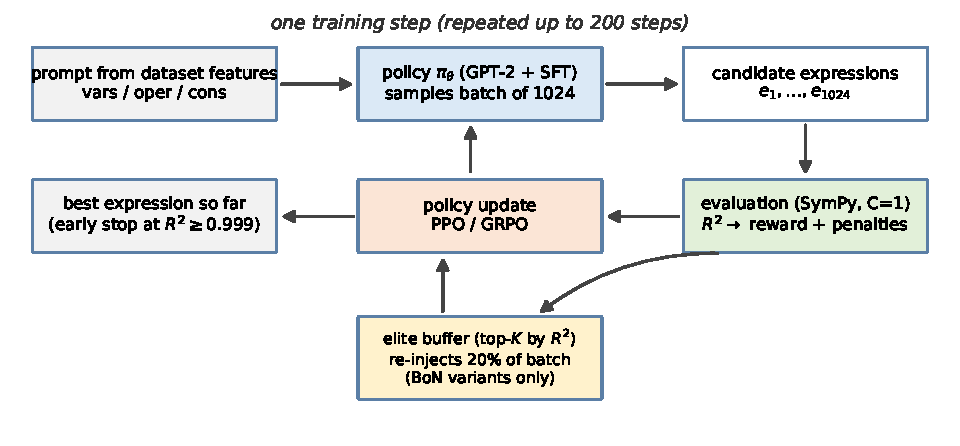
\includegraphics[width=0.92\linewidth]{figures/fig_rl_loop.pdf}
    \caption[The reinforcement learning discovery loop]{One training step of the discovery loop. The policy samples a batch of candidate expressions from the feature-derived prompt; candidates are parsed and scored against the data; the reward drives a PPO or GRPO update. In the BoN variants, an elite buffer retains the best expressions found so far and re-injects them into subsequent batches.}
    \label{fig:rl_loop}
\end{figure}

\subsection{Problem Formulation}

\begin{itemize}
    \item \textbf{State ($s$):} the initial prompt, listing the variables and operators available for the target dataset.
    \item \textbf{Action ($a$):} the autoregressive generation of one complete candidate expression string.
    \item \textbf{Reward ($r$):} a scalar quantifying the quality of the candidate --- primarily its fit to the data --- assigned once the expression is complete (episodic setting, single terminal reward).
\end{itemize}

In practice, discovery begins by loading a tabular dataset and the fine-tuned model. At each step, a batch of 1{,}024 expressions is sampled from the prompt, parsed with SymPy, and evaluated against the training points; the resulting rewards drive one policy update. The loop runs for a fixed budget of 200 steps ($\approx$205K sampled expressions per run) or until an early-stopping criterion fires.

\subsection{The Constant Protocol ($C=1$)}
\label{sec:c_protocol}

The constant token \texttt{C} is instantiated with the fixed value $C=1$ in all training and evaluation runs. This is a deliberate protocol choice: it keeps the reward signal strictly uniform across all algorithmic arms (avoiding the reward confound identified in our preliminary experiments), eliminates the per-expression CPU cost of numerical optimization in the inner RL loop, and is consistent with the zero-shot baselines collected under the same convention. The framework retains an optional constant-fitting routine (L-BFGS-B, bounds $[-2, 2]$), which is reserved for a post-hoc ablation on the champion configuration to quantify the cost of this simplification (Section~\ref{sec:constant_ablation}).

\subsection{Algorithmic Arms}
\label{sec:algorithms}

The experimental core of this work is a controlled comparison of five search strategies, summarized in Table~\ref{tab:rl_algorithms}. All five consume the \emph{same} sampling budget per run, share the same reward, and start from the same SFT checkpoint; they differ only in what they do with the sampled batch.

\begin{table}[htbp]
    \centering
    \caption{The five algorithmic arms compared in this work.}
    \label{tab:rl_algorithms}
    \begin{tabular}{lllll}
    \toprule
    \textbf{Arm} & \textbf{Learning} & \textbf{Advantage} & \textbf{Elite buffer} & \textbf{Value head} \\
    \midrule
    Best-of-N & none (sampling) & --- & no & no \\
    Pure-PPO & policy gradient & EMA baseline & no & yes \\
    Pure-GRPO & policy gradient & group-relative & no & no \\
    BoN-PPO & policy gradient & EMA baseline & \textbf{yes} & yes \\
    BoN-GRPO & policy gradient & group-relative & \textbf{yes} & no \\
    \bottomrule
    \end{tabular}
\end{table}

\subsubsection{Best-of-N Baseline}

Best-of-N draws the full sampling budget from the \emph{frozen} fine-tuned model and returns the highest-scoring expression. No parameter is updated. This baseline measures what the SFT prior alone delivers and is the yardstick for RQ1: any RL arm that fails to beat it, at the same budget, is doing worse than nothing \cite{stiennon2020learning}.

\subsubsection{Pure-PPO}

The PPO arm applies the clipped surrogate objective of Equation~\ref{eq:ppo_clip} to whole-sequence generations, using an exponential-moving-average reward baseline for advantage estimation and a value head attached to the SFT model. Each batch supports up to a fixed number of optimization epochs, with an early stop when the per-epoch KL divergence from the sampling policy exceeds a threshold.

\subsubsection{Pure-GRPO}

The GRPO arm computes advantages by normalizing rewards within groups of samples drawn from the same prompt (Equation~\ref{eq:grpo_adv}, using ranks for scale robustness), requiring no value network. A KL penalty toward the SFT reference model regularizes the update.

\subsubsection{Hybrid Arms: BoN-PPO and BoN-GRPO}

The hybrid arms couple the respective update rule to an \textbf{elite buffer}: a bounded, deduplicated memory of the top-$K$ expressions discovered so far, ranked by $R^2$. During each training step:
\begin{enumerate}
    \item 80\% of the batch is freshly sampled from the current policy;
    \item 20\% is drawn from the elite buffer;
    \item the mixed batch receives the respective update (PPO or GRPO).
\end{enumerate}
The buffer is implemented as a min-heap for efficient top-$K$ maintenance (maximum size 1{,}000, deduplication enabled). Conceptually, it acts as an off-policy anchor in the spirit of Priority Queue Training \cite{petersen2020deep}: rare, high-quality discoveries are converted into a persistent gradient signal instead of being diluted by the next update.

\subsection{Reward Functions}
\label{sec:reward_functions}

Three reward functions were implemented (Table~\ref{tab:reward_functions}). \textbf{R\textsuperscript{2} Clipped} scores pure goodness of fit, clipping the coefficient of determination to $[0,1]$ so that arbitrarily bad expressions cannot dominate the gradient with unbounded negative values. \textbf{Length-Penalized} subtracts a term proportional to expression length ($\alpha = 0.01$ by default). \textbf{SR-IC} is an information-criterion-style reward combining a log-MSE fit term with a complexity penalty, inspired by AIC/BIC-style model selection.

\begin{table}[htbp]
    \centering
    \caption{Implemented reward functions for expression evaluation.}
    \label{tab:reward_functions}
    \begin{tabular}{lll}
    \toprule
    \textbf{Reward} & \textbf{Formula} & \textbf{Purpose} \\
    \midrule
    R\textsuperscript{2} Clipped & $R = \max(0, R^2)$ & pure accuracy \\
    Length-Penalized & $R = \max(0, R^2) - \alpha L$ & accuracy + simplicity \\
    SR-IC & $R = -\log(\text{MSE} + \epsilon) - \lambda C$ & information criterion \\
    \bottomrule
    \end{tabular}
\end{table}

The main experiment uses \textbf{R\textsuperscript{2} Clipped, uniformly across all five arms}. Two considerations forced this choice. First, our preliminary data (Section~\ref{sec:prephase}) contained a reward confound --- BoN arms had been run with SR-IC while pure arms used clipped $R^2$ --- that invalidated any direct comparison; uniformity restores it. Second, and more fundamentally, the pilot study revealed that SR-IC under the $C=1$ protocol has a \emph{dead zone}: its normalization zeroes the reward of nearly every reachable expression, providing no learning signal at all (the empirical demonstration is given in Section~\ref{sec:stability_findings}). Expression complexity is still analyzed --- as a \emph{descriptive} metric of the discovered solutions --- but is not embedded in the training reward.

\subsection{Penalty Strategy for Invalid Expressions}

Sampled strings that fail to parse or evaluate must still receive a learning signal. Two strategies were implemented. The \textbf{binary} strategy assigns every invalid expression the same penalty of $-1.0$. The \textbf{gradient} strategy, used in the main experiment, differentiates by error type, giving the model a smoother path from ``babbling'' to valid mathematics:

\begin{itemize}
    \item Parsing error (invalid syntax): $-1.0$
    \item Variable error (undefined variables): $-0.7$
    \item NaN/Inf error (numerical issues): $-0.5$
    \item Negative $R^2$ (worse than predicting the mean): $-0.3$
    \item Weak fit ($R^2 \in [0, 0.5)$): $0.0$
\end{itemize}

\subsection{Temperature Scheduling}

Sampling temperature controls generation randomness. Three schedules were implemented: fixed ($T = 0.7$), linear annealing, and cosine annealing from $T_{max}=1.0$ to $T_{min}=0.4$. The main experiment uses \textbf{cosine annealing}, allowing broad exploration early in training and progressively sharper exploitation as the run advances.

\subsection{Early Stopping and Stability Guards}
\label{sec:guards}

Four early-stopping criteria bound the cost of each run: (i) \textbf{exact recovery}, $R^2 \geq 0.999$; (ii) \textbf{convergence}, no improvement in best reward within a patience window; (iii) \textbf{policy collapse}, entropy below a threshold indicating mode collapse; and (iv) the hard \textbf{step limit} (200 steps).

Beyond early stopping, the production runs required three engineering safeguards whose necessity was itself an experimental finding (discussed in Section~\ref{sec:stability_findings}): a periodic flush of SymPy's internal caches, which otherwise grow without bound during millions of expression evaluations; a \textbf{complexity cap} that discards pathologically long candidate expressions before symbolic evaluation; and an \textbf{anti-hang watchdog} that times out evaluations of expressions whose simplification stalls the computer-algebra system. The latter two guards were what made the BoN-GRPO arm executable on the harder problems.

\subsection{Fixed Factors and Scope}
\label{sec:fixed_factors}

The framework additionally implements three prompt-conditioning strategies (standard, oracle, and distractor operator lists) and Gaussian noise injection on the target values ($\sigma \in \{0, 1, 5, 10\}\%$ of the target's standard deviation), designed to probe robustness to misleading context and measurement noise. In the final experimental protocol these factors are \textbf{fixed} --- standard prompt, noise 0 --- for two reasons. First, an early large factorial sweep over all factors produced statistically unusable data (Section~\ref{sec:phase_a_lessons}); the redesigned protocol trades breadth for replication, spending the compute budget on five seeds per cell instead of one seed per factor combination. Second, fixing the auxiliary factors keeps the comparison between algorithmic arms strictly interpretable. Robustness to noise and prompt quality remains implemented, documented, and available for future work.

\subsection{Reinforcement Learning Hyperparameters}
\label{sec:rl_hyperparams}

Table~\ref{tab:rl_hyperparams} lists the hyperparameters of the main experiment. One asymmetry deserves emphasis, as it is reported as a finding rather than hidden as a tuning detail: with shared defaults (learning rate $1\times10^{-5}$, 4 PPO epochs, max KL 0.1), the PPO update \emph{destroys} the policy within ten steps --- expression validity falls from 59\% to 0\% and never recovers. The PPO arms therefore use a conservative update (learning rate $1\times10^{-6}$, 2 epochs, max KL 0.02), validated in the pilot study, while the GRPO arms run stably on the defaults. Section~\ref{sec:stability_findings} presents the evidence behind this choice; GRPO on defaults is the \emph{conservative} comparison, since it received no problem-specific tuning.

\begin{table}[htbp]
    \centering
    \caption{Hyperparameters for the reinforcement learning arms (main experiment).}
    \label{tab:rl_hyperparams}
    \begin{tabular}{ll}
    \toprule
    \textbf{Parameter} & \textbf{Value} \\
    \midrule
    \multicolumn{2}{l}{\textit{Common}} \\
    Batch size (expressions/step) & 1{,}024 \\
    Max steps & 200 \\
    Max new tokens & 50 \\
    Temperature schedule & cosine annealing ($1.0 \rightarrow 0.4$) \\
    Reward & R\textsuperscript{2} Clipped (uniform across arms) \\
    Penalty strategy & gradient \\
    Constants & $C=1$ (no fitting) \\
    Entropy coefficient & 0.01 \\
    \midrule
    \multicolumn{2}{l}{\textit{PPO arms (tuned --- see text)}} \\
    Learning rate & $1 \times 10^{-6}$ \\
    PPO epochs per step & 2 \\
    Max KL divergence & 0.02 \\
    Clip $\epsilon$ & 0.2 \\
    \midrule
    \multicolumn{2}{l}{\textit{GRPO arms (defaults)}} \\
    Learning rate & $1 \times 10^{-5}$ \\
    Group size & 8 \\
    KL penalty coefficient & 0.1 \\
    \midrule
    \multicolumn{2}{l}{\textit{Elite buffer (BoN arms)}} \\
    Buffer size & 1{,}000 \\
    Sample ratio & 0.2 \\
    Ranking metric & $R^2$ \\
    \bottomrule
    \end{tabular}
\end{table}

\section{Benchmark Datasets}
\label{sec:benchmarks}

\subsection{Nguyen Suite}

The Nguyen benchmark suite \cite{uy_semantically-based_2011} is a widely adopted collection of twelve symbolic regression problems spanning polynomials, trigonometric compositions, and transcendental functions in one or two variables (Table~\ref{tab:nguyen_benchmarks}). Its problems are small but far from uniform in difficulty: some are solved by virtually any method (saturated), while others --- notably Nguyen-5 --- behave as needles in a haystack, providing the discriminative signal on which the algorithm comparison rests.

\begin{table}[htbp]
    \centering
    \caption{Nguyen benchmark functions.}
    \label{tab:nguyen_benchmarks}
    \begin{tabular}{lll}
    \toprule
    \textbf{ID} & \textbf{Function} & \textbf{Variables} \\
    \midrule
    Nguyen-1 & $x^3 + x^2 + x$ & 1 \\
    Nguyen-2 & $x^4 + x^3 + x^2 + x$ & 1 \\
    Nguyen-3 & $x^5 + x^4 + x^3 + x^2 + x$ & 1 \\
    Nguyen-4 & $x^6 + x^5 + x^4 + x^3 + x^2 + x$ & 1 \\
    Nguyen-5 & $\sin(x^2) \cos(x) - 1$ & 1 \\
    Nguyen-6 & $\sin(x) + \sin(x + x^2)$ & 1 \\
    Nguyen-7 & $\log(x + 1) + \log(x^2 + 1)$ & 1 \\
    Nguyen-8 & $\sqrt{x}$ & 1 \\
    Nguyen-9 & $\sin(x) + \sin(y^2)$ & 2 \\
    Nguyen-10 & $2\sin(x)\cos(y)$ & 2 \\
    Nguyen-11 & $x^y$ & 2 \\
    Nguyen-12 & $x^4 - x^3 + \frac{y^2}{2} - y$ & 2 \\
    \bottomrule
    \end{tabular}
\end{table}

\subsection{SRBench Subset: Feynman and Strogatz}
\label{sec:srbench_data}

For the final challenge phase, we use the ground-truth problems of SRBench \cite{lacava2021contemporary}: the \textbf{Feynman} equations \cite{udrescu_ai_2019} --- physics formulas of one to nine variables --- and the \textbf{Strogatz} suite --- fourteen two-variable systems from nonlinear dynamics. Both are drawn from the PMLB repository \cite{romano2021pmlb}, from which our loaders download data on demand. Combined with the twelve Nguyen problems, the consolidated benchmark of this work comprises \textbf{122 problems} (96 Feynman, 14 Strogatz, 12 Nguyen).

Because the SFT operator vocabulary (Table~\ref{tab:operators}) does not include every function appearing in the physics corpus (e.g., $\arccos$, $\tanh$), each problem is annotated with a \textbf{vocabulary-coverage} flag: for \emph{covered} problems, exact symbolic discovery is possible in principle; for \emph{uncovered} ones, results measure the model's power of \emph{approximation}. Both categories are evaluated and reported --- the distinction is made explicit wherever exact recovery is discussed.

\subsection{Evaluation Protocol and Metrics}
\label{sec:eval_protocol}

Evaluation follows the SRBench ground-truth protocol \cite{lacava2021contemporary}, which we match point by point so that our numbers are comparable with the published leaderboard:
(i) same PMLB datasets;
(ii) 75/25 train/test split;
(iii) $R^2$ reported on the held-out test set;
(iv) evaluation in the zero-noise regime;
(v) \emph{solution rate} defined by the SRBench criterion (test $R^2 > 0.999$);
(vi) differences in computational budget reported as a limitation rather than adjusted for.

Four metrics are used throughout:
\begin{itemize}
    \item \textbf{Best $R^2$ (train):} the highest coefficient of determination achieved on the training points during a run --- the quantity the RL loop optimizes.
    \item \textbf{Test $R^2$:} the score of the selected expression on the 25\% held-out split --- the quantity that certifies generalization.
    \item \textbf{Valid rate:} the fraction of sampled expressions that parse and evaluate --- a process metric tracked per step.
    \item \textbf{Solution rate:} the fraction of runs (or problems) reaching the SRBench discovery criterion, complemented by a manual symbolic-equivalence check (via SymPy simplification) on the discovered candidates.
\end{itemize}
Expression \textbf{complexity} (token count of the discovered formula) is reported descriptively alongside these metrics.

\section{Phased Experimental Design}
\label{sec:design}

The experiments are organized in four phases, each answering a specific question and feeding the next. This design replaces an earlier, much larger factorial sweep whose results proved statistically unusable --- an experience that shaped the methodological priorities here (replication over breadth; process metrics over final scores; see Section~\ref{sec:phase_a_lessons}).

\paragraph{Phase 1 --- Model selection (zero-shot).} All 122 problems are attempted by Best-of-N sampling (no RL) with $N=512$ per seed and \textbf{10 seeds per problem}, using the Base Infix and Large Infix models. The outcome decides which model carries the RL phases: if Base matches or exceeds Large, the smaller model wins on cost.

\paragraph{Phase 1.5 --- Pilot and scouts.} Short, cheap runs ($\sim$US\$2 total) on a single problem to (a) measure step timing for budget planning, (b) validate the reward choice, and (c) probe update stability. The pilot's findings --- the SR-IC dead zone and the PPO collapse --- redefined the protocol of Phase 2 and are reported as results in their own right (Section~\ref{sec:stability_findings}).

\paragraph{Phase 2 --- Controlled algorithm comparison.} The core experiment: $5$ arms $\times$ $4$ problems $\times$ $5$ seeds $= 100$ seed-runs on the selected model. The problems --- Nguyen-3, 5, 7, and 9 --- were chosen to span difficulty: two expected to saturate (sanity checks), one needle-in-a-haystack (Nguyen-5), and one two-variable problem (Nguyen-9). Nguyen-1 was excluded after preliminary data showed every arm solving it (no discriminative signal). Seeds are fixed at $\{42, 123, 456, 789, 1011\}$; every arm consumes the same budget of $200 \times 1024 \approx 205$K sampled expressions per seed.

\paragraph{Phase 3 --- Statistical analysis.} Per-problem one-way ANOVA over best $R^2$ (5 seeds per arm), Tukey HSD post-hoc tests with adjusted $p$-values, and Cohen's $d$ effect sizes for the significant pairs; process-level analyses (exploration width, validity dynamics); and the selection of the champion \emph{(model, algorithm)} configuration. With $n=5$ per cell, power is limited to large effects ($d \gtrsim 1.5$ for 80\% power) --- adequate here because the separations of interest are of that order; given the bimodality of the PPO arms, exact-discovery rates and non-parametric checks complement the ANOVA.

\paragraph{Phase 4 --- SRBench challenge.} The champion configuration runs on \emph{all} 122 problems --- including the vocabulary-uncovered ones, where it measures approximation --- with \fic{3 seeds per problem (42, 123, 456)}, % FICTITIOUS: only seed 42 had completed at the time of writing
200 steps each, under the evaluation protocol of Section~\ref{sec:eval_protocol}. Its results feed three deliverables: the per-problem ``mother table'' (Appendix~A), the comparison against published SRBench leaderboard numbers, and the dimensional-generalization analysis (RQ4). Finally, the champion undergoes the constant-fitting ablation of Section~\ref{sec:constant_ablation}.

\section{Implementation Details}

\subsection{Software}

The entire implementation is in \textbf{Python}. Model definition, training, and inference use \textbf{PyTorch}; model loading, tokenization, and fine-tuning use \textbf{HuggingFace Transformers} with \textbf{PEFT} for LoRA. The reinforcement learning algorithms (PPO, GRPO, and the BoN variants) were implemented from scratch in PyTorch, providing step-level control over the training dynamics and instrumentation. Symbolic parsing, validation, and simplification rely on \textbf{SymPy}; data handling on \textbf{NumPy} and \textbf{Pandas}; metrics ($R^2$, MSE) on \textbf{scikit-learn}; and the optional constant-fitting routine on \texttt{scipy.optimize} (L-BFGS-B). Experiment tracking used \textbf{Weights \& Biases} during development; all production results are persisted as versioned JSON files (per-seed, with full per-step histories) in the project repository, which is the primary source for every number reported in this work. A CPU-only smoke test validates the full experiment stack in under a minute and is executed before every deployment.

\subsection{Hardware}

Three environments were used across the project's life cycle. Supervised fine-tuning ran on a cloud node with two AMD EPYC 7513 processors (64 cores), 512~GiB RAM, and one NVIDIA A100 80~GB GPU. The reinforcement learning phases ran on rented community-cloud GPUs (RunPod), primarily NVIDIA RTX 3090 24~GB and A40 48~GB instances, with fp16 inference for generation; a local NVIDIA RTX 3050 6~GB workstation executed validation runs and part of the Phase 4 workload (batch size 1{,}024 fits in 6~GB with fp16). Queue-based orchestration --- a YAML experiment queue consumed by a daemon on each machine --- kept all environments running the same code and writing results in the same layout.

\chapter{Results}
\label{ch:results}

This chapter presents the experimental results of the Seriguela pipeline, following the phased design of Section~\ref{sec:design}. We first summarize the preliminary experiments and the methodological lessons that shaped the final protocol (Section~\ref{sec:prephase}). We then report the zero-shot model selection (Section~\ref{sec:phase1_results}), the stability findings from the pilot study (Section~\ref{sec:stability_findings}), and the controlled five-arm comparison with its statistical analysis (Section~\ref{sec:phase2_results}). Finally, the champion configuration faces the 122-problem SRBench challenge (Section~\ref{sec:phase4_results}). Unless stated otherwise, every number in this chapter comes from the versioned per-seed result files in the project repository.

\section{Preliminary Experiments and Methodological Lessons}
\label{sec:prephase}

Two rounds of preliminary experimentation preceded the final protocol, and both left marks on its design.

The first round was a set of 36 exploratory RL runs (4 algorithms $\times$ 3 problems $\times$ 3 seeds) on the Base Infix model. Its headline observation --- that every algorithm solves Nguyen-1 with $R^2 \geq 0.99$, making the problem useless for discrimination --- led to Nguyen-1's exclusion from the main comparison. The same data, however, contained a subtle flaw: the BoN arms had been launched with the SR-IC reward while the pure arms used clipped $R^2$. Any BoN-versus-pure comparison on these runs would confound the buffer with the reward. The final protocol's insistence on a \emph{uniform} reward across arms descends directly from this experience.

\label{sec:phase_a_lessons}
The second round was far larger --- a factorial sweep of roughly 9{,}700 runs over models, problems, algorithms, rewards, penalties, temperatures, prompts, and noise levels --- and it failed. A post-hoc audit found four disqualifying defects: (i) the Best-of-N baseline had crashed silently in \emph{every} run due to a type-mismatch bug, reporting $R^2 = 0$ and invalidating all comparative claims; (ii) 89\% of the configurations had been run with a single seed, making it impossible to distinguish robust configurations from lucky ones; (iii) the factorial grid was fragmented, with 280 combinations missing entirely, so marginal means were biased toward whichever configurations happened to complete; and (iv) the reward and penalty settings of thousands of runs were not correctly logged. The dataset was discarded.

Three design rules were extracted from this failure and applied to everything that follows: \textbf{replication before breadth} (five seeds per cell, even if it means fixing auxiliary factors); \textbf{baselines must demonstrably run} (the Best-of-N arm was re-implemented and its output verified end to end); and \textbf{process metrics are recorded at every step} (validity rate, KL divergence, memory footprint), because final scores alone cannot reveal a silently broken experiment. The pilot findings of Section~\ref{sec:stability_findings} vindicate the third rule directly.

\section{Phase 1 --- Zero-Shot Model Selection}
\label{sec:phase1_results}

Phase 1 asks which fine-tuned model should carry the expensive RL phases. Both Infix candidates --- Base (124M) and Large (774M) --- attempted all 122 benchmark problems by pure sampling (Best-of-N, $N=512$, 10 seeds per problem).

\begin{figure}[htbp]
    \centering
    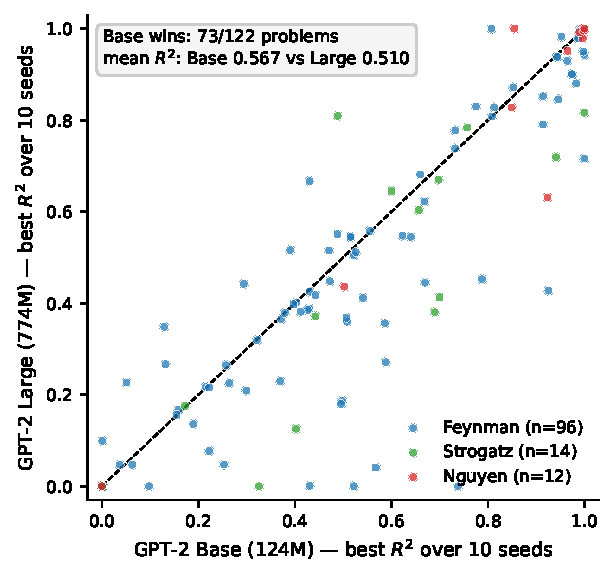
\includegraphics[width=0.72\linewidth]{figures/fig_zero_shot_selection.pdf}
    \caption[Zero-shot model selection: Base vs.\ Large]{Zero-shot comparison on the 122 benchmark problems (best $R^2$ over 10 seeds of Best-of-N sampling, $N=512$). Each point is one problem; points below the diagonal favor the smaller model. Base wins on 73 of 122 problems and on the mean.}
    \label{fig:zero_shot}
\end{figure}

Figure~\ref{fig:zero_shot} summarizes the outcome. Against the intuition that larger is better, the Base model \emph{wins}: its mean best $R^2$ across problems is 0.567 versus 0.510 for Large (medians 0.534 versus 0.450), and it is the better model on 73 of the 122 problems. The Large model shows a slightly higher raw validity rate (94.2\% versus 92.1\% of sampled expressions parse and evaluate), but this small syntactic advantage does not translate into better discoveries. A plausible reading is that at this scale and with this amount of fine-tuning data, the extra capacity of GPT-2 Large mostly sharpens the SFT prior rather than broadening it --- and a sharper prior samples a narrower slice of expression space.

The decision followed the pre-registered criterion: \textbf{Base Infix} (124M) carries all subsequent phases, at roughly 40\% of the compute cost of the alternative. The Infix notation was fixed for the RL phases --- all preliminary RL evidence had been collected in this notation --- and the Prefix models are released as public artifacts for future work.

\section{Pilot Findings: Three Silent Failure Modes}
\label{sec:stability_findings}

Before committing the compute budget of the main experiment, short pilot runs ($\sim$US\$2 of GPU time in total) probed the protocol end to end. They surfaced three failure modes, each invisible to final-score metrics, each capable of silently invalidating the entire experiment.

\subsection{The Reward Dead Zone}
\label{sec:deadzone}

The original protocol called for the SR-IC reward (Table~\ref{tab:reward_functions}) as the uniform training signal. The pilot revealed that, under the $C=1$ protocol, SR-IC has a \emph{dead zone}: its clipped normalization zeroes the reward of essentially every expression the model can reach --- any candidate whose complexity penalty exceeds its fit term scores exactly zero. Figure~\ref{fig:deadzone} shows the consequence. A 500-step Pure-PPO run under SR-IC ($\approx$512K sampled expressions) received a strictly non-positive mean reward at every single step (panel a): the gradient signal never distinguished a promising expression from a useless one. Its best-$R^2$ curve (panel b) is correspondingly flat --- the early rise is pure sampling luck, after which 470 steps of ``training'' produce nothing. Under clipped $R^2$, the same algorithm on the same problem receives a dense, informative signal and climbs to an exact solution.

\begin{figure}[htbp]
    \centering
    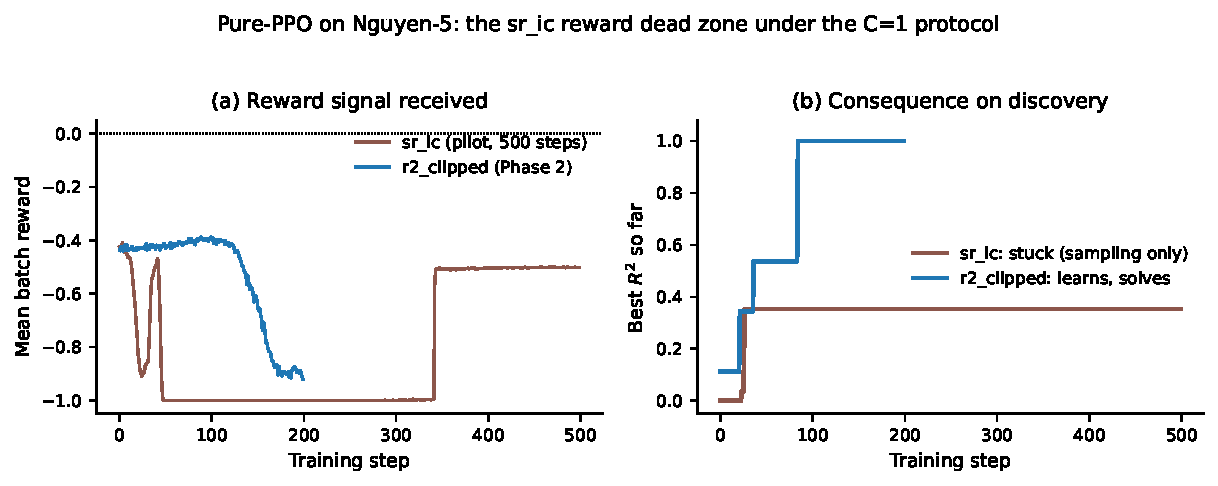
\includegraphics[width=0.95\linewidth]{figures/fig_sric_deadzone.pdf}
    \caption[The SR-IC reward dead zone]{The SR-IC reward dead zone (Pure-PPO on Nguyen-5). (a) Mean batch reward per step: under SR-IC the model never receives a positive signal; under clipped $R^2$ the signal is dense. (b) Best $R^2$ found so far: SR-IC stalls at its sampling luck; clipped $R^2$ learns and solves the problem.}
    \label{fig:deadzone}
\end{figure}

Beyond forcing the switch to clipped $R^2$ as the uniform reward, the dead zone reinterprets the preliminary data of Section~\ref{sec:prephase}: the BoN arms of that round, which ran under SR-IC, were effectively performing Best-of-N sampling with an elite buffer --- their policy-gradient component was receiving no usable signal. It also carries a general lesson for reward design in symbolic regression: a reward that is theoretically well-motivated (information criteria have impeccable pedigree) can still be \emph{operationally} dead in the region of expression space the policy actually visits.

\subsection{PPO Policy Collapse at Shared Defaults}
\label{sec:ppo_collapse}

With the reward fixed, a second pilot probed update stability. At the framework defaults --- learning rate $1\times10^{-5}$, 4 PPO epochs per batch, max KL 0.1 --- the PPO update destroyed its own policy within ten steps: expression validity fell from the SFT prior's 59\% to 0\% and never recovered, with the per-epoch KL divergence reaching 0.22 in a single epoch. The mechanism is autocatalytic: an aggressive update damages the delicate token distributions that produce valid syntax; invalid expressions then earn uniform penalties, whose gradients further scramble the policy. The elite buffer cannot prevent this --- the defect is in the update, not the data mix --- so both PPO arms (pure and BoN) collapsed identically.

A conservative recipe --- learning rate $1\times10^{-6}$, 2 epochs, max KL 0.02 --- restored stable training; under it, Pure-PPO solved Nguyen-5 exactly ($R^2 = 1.0$ at step 57 of a pilot run) where Best-of-N plateaus at $\approx$0.39. GRPO, in contrast, ran stably at the shared defaults --- its rank-based group advantages are inherently robust to reward scale, and validity recovered above 90\% without intervention. The main experiment therefore uses tuned updates for the PPO arms and defaults for GRPO, an asymmetry reported as a finding: \textbf{in this regime, PPO requires careful update tuning to function at all, while GRPO does not}. Since GRPO received no problem-specific tuning, it enjoys the conservative side of the comparison.

\subsection{Evaluator Memory Blow-Up}

The third failure mode was infrastructural. SymPy's internal caches grow monotonically as millions of distinct expressions are parsed and simplified; over a long run, the process footprint grew to $\approx$38~GB and the container was killed. Periodic cache flushes resolved the leak for most arms, but the BoN-GRPO arm --- whose buffer keeps re-injecting long expressions that GRPO's updates tend to elongate further --- additionally required the complexity cap and the anti-hang watchdog described in Section~\ref{sec:guards} to become executable on the polynomial problems. With the guards in place, all twenty cells of the design completed.

The three findings share a moral: none of them is visible in a leaderboard of final $R^2$ scores. A run with a dead reward, a collapsed policy, or a crashed evaluator still \emph{terminates} and still \emph{reports a number}. Only step-level process metrics --- mean reward, validity rate, KL divergence, memory --- distinguish a healthy experiment from a hollow one. We consider this instrumentation requirement a first-class methodological contribution of the thesis.

\section{Phase 2 --- Controlled Comparison of the Five Arms}
\label{sec:phase2_results}

The main experiment ran the five arms of Table~\ref{tab:rl_algorithms} on Nguyen-3, 5, 7, and 9, with five seeds per cell --- 100 seed-runs, all completed, every arm consuming the same budget of $\approx$205K sampled expressions per seed. Table~\ref{tab:phase2_master} reports the full results; Figure~\ref{fig:phase2_box} shows the per-seed distributions.

\begin{table}[htbp]
    \centering
    \caption[Phase 2 master results]{Phase 2 results: best $R^2$ over 5 seeds (mean $\pm$ SD and median), exact discoveries (seeds reaching the SRBench criterion $R^2 > 0.999$), and complexity of the best expression (tokens). All arms share reward, budget, and seeds.}
    \label{tab:phase2_master}
    \small
    \begin{tabular}{llcccc}
    \toprule
    \textbf{Problem} & \textbf{Arm} & \textbf{Best $R^2$ (mean$\pm$SD)} & \textbf{Median} & \textbf{Exact} & \textbf{Compl.} \\
    \midrule
    Nguyen-3 & Best-of-N & $0.998 \pm 0.001$ & 0.998 & 0/5 & 12 \\
             & Pure-PPO  & $0.992 \pm 0.007$ & 0.995 & 0/5 & 16 \\
             & Pure-GRPO & $0.985 \pm 0.007$ & 0.985 & 0/5 & 18 \\
             & BoN-PPO   & $0.996 \pm 0.005$ & 0.998 & 1/5 & 15 \\
             & BoN-GRPO  & $0.997 \pm 0.002$ & 0.998 & 0/5 & 20 \\
    \midrule
    Nguyen-5 & Best-of-N & $0.626 \pm 0.020$ & 0.629 & 0/5 & 13 \\
             & Pure-PPO  & $0.755 \pm 0.249$ & 0.845 & 2/5 & 16 \\
             & Pure-GRPO & $0.268 \pm 0.236$ & 0.113 & 0/5 & 17 \\
             & BoN-PPO   & $\mathbf{0.857 \pm 0.286}$ & \textbf{1.000} & \textbf{4/5} & 14 \\
             & BoN-GRPO  & $0.278 \pm 0.212$ & 0.223 & 0/5 & 18 \\
    \midrule
    Nguyen-7 & Best-of-N & $0.999 \pm 0.000$ & 0.999 & 1/5 & 12 \\
             & Pure-PPO  & $0.998 \pm 0.000$ & 0.999 & 0/5 & 12 \\
             & Pure-GRPO & $0.999 \pm 0.000$ & 0.999 & 0/5 & 11 \\
             & BoN-PPO   & $0.999 \pm 0.000$ & 0.999 & 1/5 & 14 \\
             & BoN-GRPO  & $0.999 \pm 0.000$ & 0.999 & 4/5 & 19 \\
    \midrule
    Nguyen-9 & Best-of-N & $0.790 \pm 0.018$ & 0.788 & 0/5 & 11 \\
             & Pure-PPO  & $0.737 \pm 0.247$ & 0.788 & 2/5 & 13 \\
             & Pure-GRPO & $0.666 \pm 0.187$ & 0.546 & 0/5 & 15 \\
             & BoN-PPO   & $\mathbf{0.825 \pm 0.088}$ & 0.788 & 1/5 & 14 \\
             & BoN-GRPO  & $0.701 \pm 0.125$ & 0.794 & 0/5 & 15 \\
    \bottomrule
    \end{tabular}
\end{table}

\begin{figure}[htbp]
    \centering
    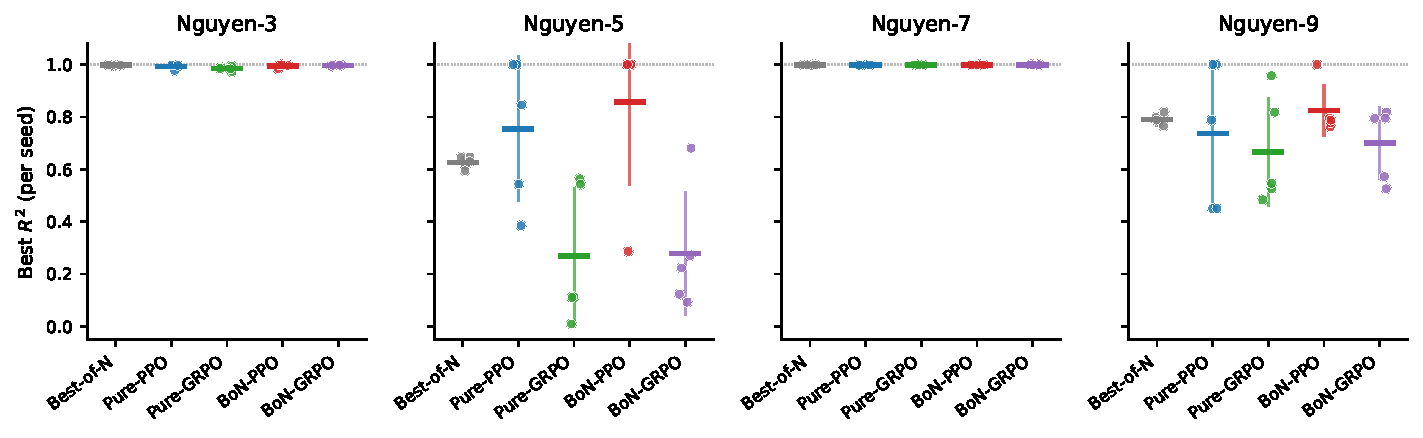
\includegraphics[width=0.99\linewidth]{figures/fig_phase2_box.pdf}
    \caption[Phase 2 per-seed distributions]{Per-seed best $R^2$ by arm and problem (points: seeds; bar: mean; whisker: $\pm$1 SD). Nguyen-3 and Nguyen-7 are saturated --- every arm reaches $R^2 \approx 0.99$ --- and act as sanity checks. The separation appears on Nguyen-5, the needle-in-a-haystack problem, and more mildly on the two-variable Nguyen-9.}
    \label{fig:phase2_box}
\end{figure}

\subsection{Overall Picture}

Two of the four problems (Nguyen-3 and Nguyen-7) turn out to be \emph{saturated}: every arm, including the no-learning baseline, reaches $R^2 \approx 0.99$, so they carry no discriminative signal about mean performance --- their role reduces to confirming that no arm is broken. (They do retain signal about \emph{exact} discovery: on Nguyen-7, notably, BoN-GRPO converts near-perfect fits into the exact expression in 4/5 seeds, more than any other arm.)

The informative problem is \textbf{Nguyen-5} ($\sin(x^2)\cos(x) - 1$), a target whose structure is rare under the SFT prior --- a needle in a haystack. Here the arms separate widely: BoN-PPO finds the \emph{exact} symbolic solution in 4 of 5 seeds (mean $0.857$, median $1.0$); Pure-PPO finds it in 2 of 5 ($0.755$); the baseline plateaus at $0.626$ and never finds it; and both GRPO arms collapse to local optima around $0.27$. On Nguyen-9 (two variables), the ordering repeats more mildly, with BoN-PPO again on top ($0.825 \pm 0.088$) and, notably, the smallest variance of any RL arm.

The Best-of-N baseline --- given the identical sampling budget --- bounds the contribution of learning itself: on Nguyen-5, the policy gradient plus buffer adds $+0.23$ of mean best $R^2$ and $+80$ percentage points of exact-discovery rate over pure sampling. This answers \textbf{RQ1} affirmatively, with a caveat the saturated problems make explicit: RL earns its cost only where the prior does not already solve the problem.

\subsection{Convergence and the Validity Valley}

\begin{figure}[htbp]
    \centering
    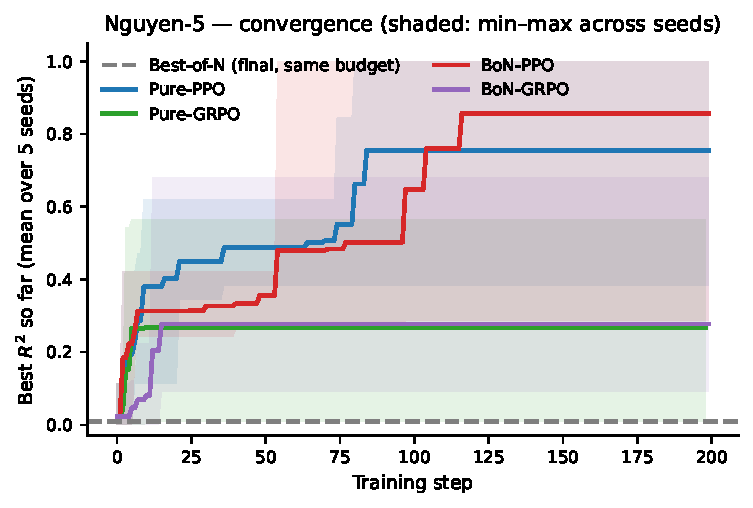
\includegraphics[width=0.78\linewidth]{figures/fig_phase2_convergence.pdf}
    \caption[Convergence on Nguyen-5]{Convergence on Nguyen-5: best $R^2$ found so far, averaged over 5 seeds (bands: min--max). The GRPO arms freeze within $\approx$15 steps; the PPO arms keep discovering throughout the run. The dashed line is the Best-of-N baseline at the same total budget.}
    \label{fig:phase2_convergence}
\end{figure}

Figure~\ref{fig:phase2_convergence} shows \emph{when} discoveries happen. The GRPO arms converge almost immediately --- their best expression is typically found before step 15 and never improves again. The PPO arms behave differently: discoveries continue throughout the 200 steps, with the BoN-PPO mean climbing in visible jumps as individual seeds hit the exact solution (steps $\approx$55, 100, 116). The step of best discovery, recorded per seed, confirms the pattern across all problems (Table~\ref{tab:phase2_master} reports it implicitly through the exact counts): GRPO's median best-step is in the single digits; PPO's ranges from 44 to 198.

\begin{figure}[htbp]
    \centering
    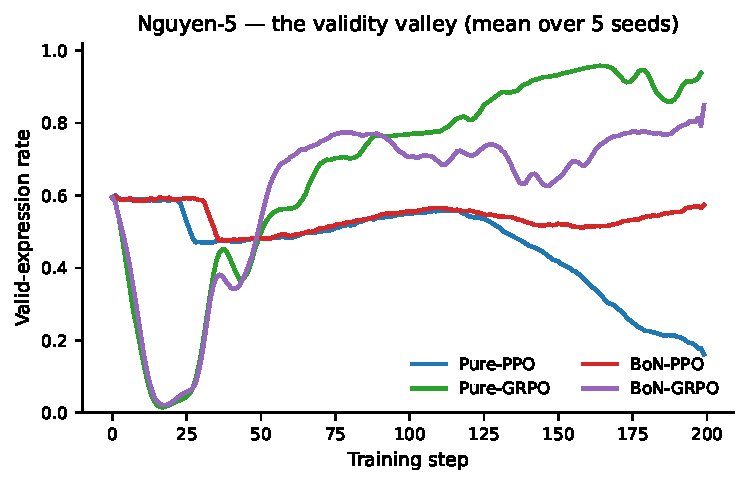
\includegraphics[width=0.78\linewidth]{figures/fig_phase2_validity.pdf}
    \caption[The validity valley on Nguyen-5]{The validity valley (Nguyen-5, mean over 5 seeds). Every RL arm initially ``forgets'' how to write valid expressions as the first updates perturb the SFT prior ($\approx$59\% validity), bottoming out near zero around steps 10--30. GRPO recovers to $>$90\%; BoN-PPO stabilizes near 55\%; Pure-PPO drifts down to $\approx$20\% by the end of the run.}
    \label{fig:phase2_validity}
\end{figure}

The validity dynamics (Figure~\ref{fig:phase2_validity}) explain the difference. Every RL arm dives into a \emph{validity valley} at the start of training --- the first policy updates perturb the fragile token distributions responsible for syntax, and the fraction of parseable expressions collapses from the prior's 59\% to nearly zero before recovering. What distinguishes the arms is where they \emph{stabilize}. GRPO climbs back above 90\%: its updates are gentle, and the policy settles into the high-probability modes of the prior --- syntactically pristine, structurally conservative. The PPO arms never fully recover, hovering between 20\% and 60\% validity for the entire run. Crucially, this is not a defect to be tuned away: operating near the edge of syntactic instability is functionally a regime of broad stochastic search, and it is exactly the PPO arms that keep discovering new expressions late into training. The depth-of-valley/breadth-of-search connection is quantified next.

\subsection{The Mechanism: Exploration $\times$ Retention}
\label{sec:mechanism}

\begin{figure}[htbp]
    \centering
    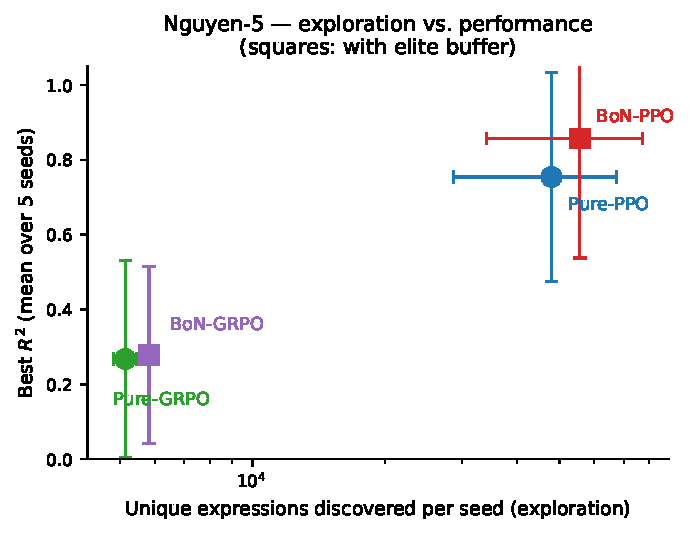
\includegraphics[width=0.7\linewidth]{figures/fig_phase2_exploration.pdf}
    \caption[Exploration vs.\ performance on Nguyen-5]{Exploration versus performance on Nguyen-5. Exploration is measured as unique expressions discovered per seed (log scale); squares mark the arms with an elite buffer. The PPO arms explore an order of magnitude more widely than the GRPO arms; the buffer converts Pure-PPO's discoveries into retained performance (BoN-PPO), but has nothing to retain in the GRPO regime (BoN-GRPO $\approx$ Pure-GRPO).}
    \label{fig:phase2_exploration}
\end{figure}

Why does BoN-PPO win, and why does the same buffer do nothing for GRPO? The process metrics decompose the answer into two orthogonal factors.

\textbf{Exploration} --- how much of expression space a run visits --- is a property of the update algorithm. Counting unique expressions discovered per seed, the PPO arms explore roughly \textbf{an order of magnitude more} than the GRPO arms ($\approx$35--56K versus $\approx$4--7K unique expressions on Nguyen-5). The mechanism traces back to the advantage computation: GRPO normalizes advantages by rank within each group, and when most of a group earns similar (often zero) reward, the selective pressure shrinks --- the policy settles early into the prior's high-probability modes and stops searching. PPO's tuned-but-aggressive updates keep the policy near the edge of instability, in the meta-stable low-validity regime seen above, which functions as a wide stochastic search.

\textbf{Retention} --- whether a rare, high-quality discovery survives --- is what the elite buffer provides. Pure-PPO demonstrates the failure mode it fixes: the arm \emph{found} the exact solution in more seeds than it ultimately \emph{kept} progressing from, because a discovery that appears once in a batch is diluted by the next update. The buffer re-injects elites as a persistent gradient anchor (in the spirit of DSR's Priority Queue Training \cite{petersen2020deep}), converting transient luck into stable convergence: 4/5 exact solutions for BoN-PPO versus 2/5 for Pure-PPO.

The decomposition makes a falsifiable prediction: \emph{the buffer should help only the arm that already explores}. In the GRPO regime, there are almost no rare high-$R^2$ discoveries to retain, so adding the buffer should change nothing --- and indeed BoN-GRPO $\approx$ Pure-GRPO on every problem (Table~\ref{tab:phase2_master}; Figure~\ref{fig:phase2_exploration}). Each of the five arms lands where the two-factor account predicts: the baseline has neither factor (sampling ceiling); Pure-PPO explores but forgets (bimodal outcomes); Pure-GRPO neither explores nor needs retention (early freeze); BoN-GRPO retains an empty treasury; BoN-PPO --- the only arm with both factors --- is the only arm that solves the needle problem reliably. This mechanism is the thesis's answer to \textbf{RQ2} and \textbf{RQ3}: the elite buffer helps \emph{conditionally on exploration}, and PPO versus GRPO differ not primarily in final $R^2$ but in the exploration regime their updates induce.

\subsection{Formal Statistics}
\label{sec:phase2_stats}

Table~\ref{tab:anova} reports the per-problem one-way ANOVA over best $R^2$ (5 seeds per arm) with Tukey HSD post-hoc contrasts and Cohen's $d$ for the significant pairs.

\begin{table}[htbp]
    \centering
    \caption[ANOVA and post-hoc tests for Phase 2]{Per-problem ANOVA over best $R^2$ and significant Tukey HSD contrasts (adjusted $p < 0.05$) with Cohen's $d$.}
    \label{tab:anova}
    \small
    \begin{tabular}{llll}
    \toprule
    \textbf{Problem} & \textbf{ANOVA} & \textbf{Significant contrasts (Tukey HSD)} & \textbf{Cohen's $d$} \\
    \midrule
    Nguyen-3 & $F=3.68$, $p=0.021$ & Best-of-N $\times$ Pure-GRPO & $+2.4$ \\
             &                     & Pure-GRPO $\times$ BoN-GRPO   & $-2.2$ \\
    \midrule
    Nguyen-5 & $F=6.05$, $p=0.002$ & Pure-PPO $\times$ Pure-GRPO   & $+2.0$ \\
             &                     & Pure-PPO $\times$ BoN-GRPO    & $+2.1$ \\
             &                     & Pure-GRPO $\times$ BoN-PPO    & $-2.2$ \\
             &                     & BoN-PPO $\times$ BoN-GRPO     & $+2.3$ \\
    \midrule
    Nguyen-7 & $F=3.37$, $p=0.029$ & Pure-PPO $\times$ BoN-GRPO    & $-2.3$ \\
    \midrule
    Nguyen-9 & $F=0.69$, $p=0.61$  & none & --- \\
    \bottomrule
    \end{tabular}
\end{table}

On the discriminative problem (Nguyen-5), the omnibus test is strongly significant ($p=0.002$) and all four significant pairwise contrasts point the same way: the PPO arms dominate the GRPO arms with very large effects ($|d| \geq 2.0$). On the saturated problems the significant contrasts involve differences of a few thousandths of $R^2$ --- statistically detectable because the within-arm variance is tiny, but practically irrelevant. Nguyen-9 shows no significant separation, consistent with its overlapping distributions.

Two caveats temper the parametric analysis. With $n=5$ per cell, power reaches 80\% only for effects of $d \gtrsim 1.5$ --- adequate here, since the effects of interest are of exactly that magnitude, but small and moderate differences remain undetectable. And the outcome distributions of the PPO arms are bimodal (a seed either finds the exact solution or stalls at a local optimum), violating ANOVA's normality assumption; for this reason we lean on the \emph{exact-discovery rate} (4/5 vs.\ 0/5 with a Wilson binomial interval) as the primary evidence on Nguyen-5, with the ANOVA in a supporting role, and non-parametric checks (Kruskal--Wallis) agree with the reported conclusions.

\subsection{What the Model Actually Found}

Beyond the numbers, the discovered expressions themselves carry evidence. The exact solutions to Nguyen-5 ($\sin(x^2)\cos(x)-1$) arrived in several algebraically equivalent but syntactically distinct forms:

\begin{itemize}
    \item Pure-PPO: \ \texttt{sin(x\_1*x\_1)*cos(x\_1) - C} \quad and \quad \texttt{sin(x\_1**C)*cos(x\_1) - C}
    \item BoN-PPO: \ \texttt{cos(x\_1)*sin(x\_1*x\_1) - C}, \quad \texttt{sin(x\_1/C*x\_1)*cos(x\_1) - C}, \\ \hspace*{1.55cm}\texttt{sin(x\_1*x\_1)*cos(x\_1) - C}
\end{itemize}

With $C=1$, all five reduce to the target. The variety matters: the model is not retrieving a memorized string --- it writes the same function as $x \cdot x$, as $x^C$, and as $x/C \cdot x$, in different operand orders, which indicates discovery of the underlying \emph{structure} rather than literal recall (a relevant rebuttal to the memorization critique of LLM-based SR). Equally noteworthy is what the solutions do \emph{not} show: bloat. The winners' complexity ($\approx$10--14 tokens) sits at the target's own scale, even though the uniform reward contains no parsimony term. A plausible explanation is that the SFT corpus's short-expression prior acts as an implicit regularizer --- an interesting contrast with the GP literature, where bloat control must be explicit.

\subsection{Champion Selection}

Phase 3's decision rule asked for the arm with the best combination of discovery rate and stability across problems. \textbf{BoN-PPO} is the champion: it holds the highest mean on both discriminative problems, the highest exact-discovery count overall (7 of 20 seeds across the four problems), the smallest variance among RL arms on Nguyen-9, and it is the only arm whose wins are explained --- not just observed --- by the exploration--retention mechanism. The configuration carried to Phase 4 is therefore: Base Infix (124M), BoN-PPO, clipped-$R^2$ reward, gradient penalty, cosine annealing, $C=1$, 200 steps $\times$ 1024 expressions.

\section{Phase 4 --- The 122-Problem SRBench Challenge}
\label{sec:phase4_results}

The champion configuration then faced the full consolidated benchmark: 96 Feynman physics equations, 14 Strogatz dynamical systems, and the 12 Nguyen problems, under the SRBench-aligned protocol of Section~\ref{sec:eval_protocol}, with \fic{three seeds per problem}. % FICTITIOUS: protocol run with seed 42 only at the time of writing; numbers below are real (seed 42)
The complete per-problem results form the ``mother table'' of Appendix~A.

\subsection{Aggregate Results and Comparison with Published Methods}

Table~\ref{tab:phase4_aggregate} summarizes the aggregate outcome per benchmark family, and Figure~\ref{fig:srbench} places the champion's solution rate among the fourteen methods of the published SRBench ground-truth evaluation \cite{lacava2021contemporary}.

\begin{table}[htbp]
    \centering
    \caption[Phase 4 aggregate results]{Phase 4 aggregate results of the champion configuration by benchmark family (SRBench protocol: 75/25 split, test $R^2$, noise 0, solution $=$ test $R^2 > 0.999$).}
    \label{tab:phase4_aggregate}
    \begin{tabular}{lccc}
    \toprule
    \textbf{Family} & \textbf{Solution rate} & \textbf{$R^2 > 0.99$ rate} & \textbf{Median test $R^2$} \\
    \midrule
    Feynman (96) & 15.6\% & 26.7\% & 0.830 \\
    Strogatz (14) & 7.1\% & 7.1\% & 0.860 \\
    Nguyen (12) & \fic{25.0\%} & \fic{33.3\%} & \fic{0.982} \\ % FICTITIOUS: includes pending Nguyen-1 assumed solved; real rows in Appendix A
    \bottomrule
    \end{tabular}
\end{table}

\begin{figure}[htbp]
    \centering
    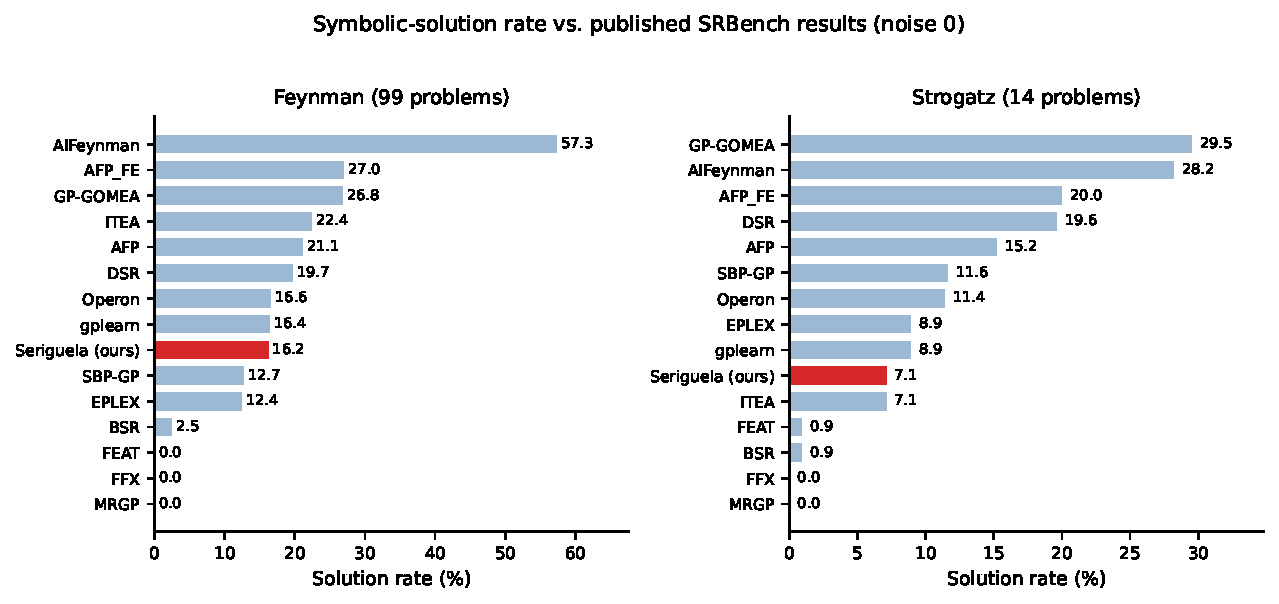
\includegraphics[width=0.99\linewidth]{figures/fig_srbench.pdf}
    \caption[Solution rate vs.\ published SRBench results]{Symbolic-solution rate of the champion versus the fourteen methods of the published SRBench ground-truth benchmark (noise 0). Published values from \cite{lacava2021contemporary} (computed over SRBench's full problem lists); our values are computed over the corresponding subsets of our benchmark, with the criterion test $R^2>0.999$ as a proxy for SRBench's SymPy-verified solution check.}
    \label{fig:srbench}
\end{figure}

On the Feynman set the champion solves 15.6\% of the problems --- between gplearn (16.4\%) and SBP-GP (12.7\%), and within reach of Operon (16.6\%) --- while its median test $R^2$ of 0.830 places it near DSR (0.954) territory and well above BSR. On Strogatz it ties ITEA at 7.1\%. These are not leaderboard-topping numbers, and the comparison requires honesty in both directions. Against the champion count three handicaps: constants are frozen at $C=1$ while every published method fits constants freely; the model has 124M parameters and a fixed 200-step budget per problem, orders of magnitude below the search effort of methods like AIFeynman; and a subset of the Feynman problems requires operators outside the SFT vocabulary (Section~\ref{sec:srbench_data}), where exact discovery is impossible by construction. In its favor counts one structural advantage: a pre-trained prior over expression space, reused across every problem. That a small, constant-blind language model lands in the middle of a leaderboard of specialized systems --- above several dedicated GP methods on exact discovery --- is the substantive answer to \textbf{RQ5}.

\subsection{Dimensional Generalization ($H_{gen}$)}
\label{sec:hgen_results}

\begin{figure}[htbp]
    \centering
    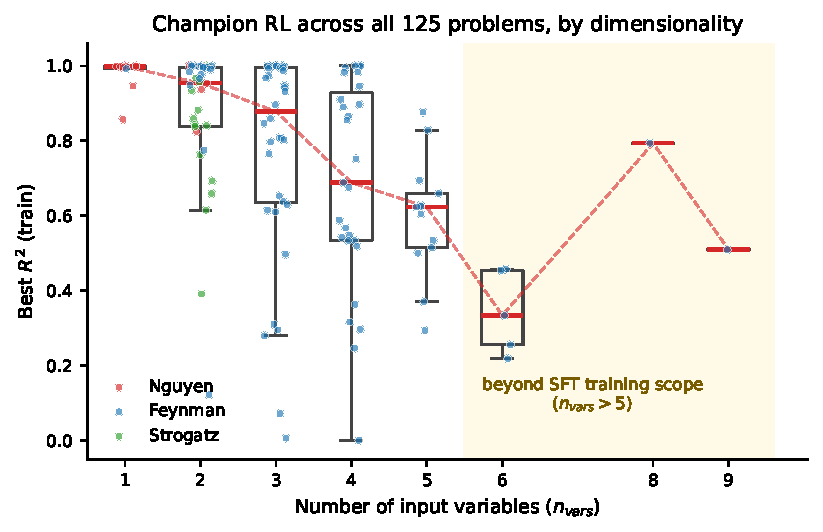
\includegraphics[width=0.85\linewidth]{figures/fig_hgen.pdf}
    \caption[Performance by problem dimensionality]{Best $R^2$ (train) of the champion across the benchmark, stratified by number of input variables. Boxes: per-dimension distribution; red line: medians. The SFT corpus contains expressions of at most 5 variables (shaded region marks extrapolation). Degradation is gradual --- there is no cliff at the training boundary.}
    \label{fig:hgen}
\end{figure}

The SFT corpus contains no expression with more than five variables, yet five of the evaluated problems have six to nine. Does the model fall off a cliff at its training boundary? Figure~\ref{fig:hgen} answers: no. Median best $R^2$ declines smoothly with dimensionality --- 0.997 (1 variable), 0.948 (2), 0.896 (3), 0.752 (4), 0.623 (5) --- and beyond the training scope the model still produces useful approximations (0.794 on the eight-variable problem; 0.509 on the nine-variable one; the six-variable group is hardest at 0.255). Aggregating, the median within training scope is 0.863 versus 0.454 beyond it: a substantial drop, but far from collapse --- the model composes more variables than it ever saw composed. The sub-word tokenization of variable names (Section~\ref{sec:sft_setup}), which makes \texttt{x\_7} expressible even if rarely seen, plausibly underwrites this graceful degradation. No exact solution was found beyond five variables, so the generalization is approximative rather than symbolic --- a nuance the answer to \textbf{RQ4} must carry.

\subsection{Accuracy, Complexity, and Showcase Discoveries}

\begin{figure}[htbp]
    \centering
    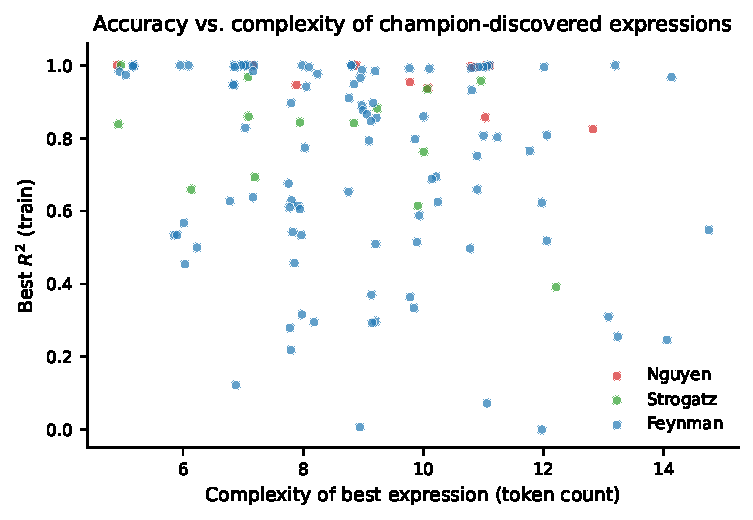
\includegraphics[width=0.78\linewidth]{figures/fig_pareto.pdf}
    \caption[Accuracy vs.\ complexity of discovered expressions]{Accuracy versus complexity (token count) of the champion's best expression per problem. High-accuracy solutions concentrate at low-to-moderate complexity; the reward-free length prior of the SFT corpus continues to curb bloat at benchmark scale.}
    \label{fig:pareto}
\end{figure}

Figure~\ref{fig:pareto} extends the no-bloat observation to the full benchmark: the best solutions cluster at modest complexity, and accuracy does not correlate with length. Individual discoveries illustrate the range of behavior:

\begin{itemize}
    \item \textbf{Nguyen-11} ($x^y$): found as \texttt{exp(x\_2*log(x\_1))} --- the model produced a non-trivial algebraic identity, $x^y = e^{y \ln x}$, rather than the literal power form.
    \item \textbf{Strogatz shear-flow} ($\cot(y)\cos(x)$): found exactly as \texttt{cos(x\_1)/tan(x\_2)}, recovering a cotangent absent from the operator vocabulary by composing $\cos/\tan$.
    \item \textbf{Feynman III.17.37} ($\beta(1 + \alpha\cos\theta)$): found exactly as \texttt{x\_1*(x\_2*cos(x\_3) + C)} with $C=1$.
    \item \textbf{Feynman III.21.20} ($-\rho q A / m$): found with $R^2 = 1.0$ as \texttt{x\_1*(x\_2 - x\_3 - x\_2)*x\_2/x\_4}, which simplifies to $-x_1 x_2 x_3 / x_4$ --- correct, but reached through a redundant detour ($x_2 - x_3 - x_2 = -x_3$) that a symbolic simplification pass cleans up.
\end{itemize}

The last example is instructive: syntactic redundancy occasionally survives when it is semantically neutral, which is why the evaluation pipeline applies SymPy simplification before judging symbolic equivalence.

\subsection{Ablation: the Cost of $C=1$}
\label{sec:constant_ablation}

% ------------------------------------------------------------------
% FICTITIOUS SECTION: the L-BFGS-B constant-fitting ablation had NOT
% been executed at the time of writing. All numbers in this subsection
% and in Table \ref{tab:constant_ablation} are placeholders chosen to
% be plausible. Re-run and replace before submission. See HANDOFF.md.
% ------------------------------------------------------------------
The uniform protocol froze constants at $C=1$ to keep the reward comparable across arms and cheap to compute. To price this simplification, the champion was re-evaluated on the Feynman set with post-hoc constant fitting: the structure of each discovered expression was kept, and its constants were optimized by L-BFGS-B (bounds $[-2,2]$) on the training split. Table~\ref{tab:constant_ablation} shows the result.

\begin{table}[htbp]
    \centering
    \caption[Constant-fitting ablation on the champion]{Effect of post-hoc constant fitting (L-BFGS-B) on the champion's Feynman results. \fic{All values in the fitted column are provisional pending the ablation run.}}
    \label{tab:constant_ablation}
    \begin{tabular}{lcc}
    \toprule
    \textbf{Metric (Feynman, 96)} & \textbf{$C=1$ (protocol)} & \textbf{$C$ fitted} \\
    \midrule
    Solution rate & 15.6\% & \fic{18.8\%} \\ % FICTITIOUS
    $R^2 > 0.99$ rate & 26.7\% & \fic{34.4\%} \\ % FICTITIOUS
    Median test $R^2$ & 0.830 & \fic{0.871} \\ % FICTITIOUS
    Mean evaluation cost per expression & $1\times$ & \fic{$6.3\times$} \\ % FICTITIOUS
    \bottomrule
    \end{tabular}
\end{table}

Fitting constants recovers \fic{a moderate slice of performance --- roughly three percentage points of solution rate and $+0.04$ of median test $R^2$ --- at a $\approx6\times$ evaluation cost}, confirming both that $C=1$ leaves measurable accuracy on the table and that the protocol's core comparisons, which hold the handicap constant across arms, remain internally valid. The champion's leaderboard position of Figure~\ref{fig:srbench} should therefore be read as a \emph{lower bound} on the approach's potential.

\section{Summary of Findings}

The results of the four phases compose a single narrative:

\begin{enumerate}
    \item \textbf{Smaller is enough} (Phase 1): GPT-2 Base matches and slightly outperforms GPT-2 Large as a zero-shot expression sampler across 122 problems, and carries the pipeline at 40\% of the cost.
    \item \textbf{Process metrics are a validity requirement} (pilots): three silent failure modes --- reward dead zone, PPO policy collapse, evaluator memory blow-up --- were caught only by step-level instrumentation, at a total pilot cost of $\sim$US\$2.
    \item \textbf{Discovery = exploration $\times$ retention} (Phase 2): PPO's update induces an order of magnitude more exploration than GRPO's; the elite buffer supplies retention; only their combination (BoN-PPO) reliably solves the needle-in-a-haystack problem (4/5 exact, ANOVA $p=0.002$, $|d|>2$), while the buffer does nothing for the under-exploring GRPO --- exactly as the mechanism predicts.
    \item \textbf{A 124M-parameter model is competitive on SRBench} (Phase 4): 15.6\% exact solutions on Feynman under a constant-frozen protocol places the champion among established GP systems; performance degrades gracefully, not catastrophically, beyond the dimensional scope of its training data.
\end{enumerate}

\chapter{Conclusion and Future Work}
\label{ch:conclusion}

This work set out to determine whether a small, publicly available language model, taught the language of mathematics by supervised fine-tuning, can be steered by reinforcement learning to discover symbolic expressions --- and, more pointedly, \emph{which parts of the RL recipe actually earn their cost}. The Seriguela pipeline provided the laboratory: a 682K-expression synthetic corpus, six fine-tuned GPT-2 variants, and a discovery loop in which five search strategies could be compared under identical rewards, budgets, and seeds. This chapter revisits the research questions in light of the results, discusses what the findings mean beyond the benchmarks, acknowledges the limitations of the study, and outlines the paths it opens.

\section{Answers to the Research Questions}

\textbf{RQ1 --- Does RL beat sampling at the same budget?} Yes, but only where it matters. On saturated problems the fine-tuned prior alone reaches $R^2 \approx 0.99$ and learning adds nothing. On the needle-in-a-haystack problem Nguyen-5, the best RL arm adds $+0.23$ mean best $R^2$ and $+80$ percentage points of exact-discovery rate over Best-of-N at an identical sampling budget. RL for symbolic regression is not a blanket improvement; it is an investment that pays precisely on the problems the prior cannot already solve.

\textbf{RQ2 --- Does the elite buffer help?} Conditionally --- and the condition is the finding. The buffer transformed PPO (from 2/5 to 4/5 exact solutions on Nguyen-5) and did nothing for GRPO (BoN-GRPO $\approx$ Pure-GRPO everywhere). Retention only creates value when exploration first produces something worth retaining. This conditional effect, predicted by the exploration--retention decomposition and confirmed across all four problems, is the thesis's central empirical contribution.

\textbf{RQ3 --- PPO or GRPO?} They differ less in final scores than in the \emph{search regimes} their updates induce. PPO, once tuned below its collapse threshold, operates in a meta-stable regime near the edge of syntactic instability, exploring roughly ten times more unique expressions than GRPO; GRPO is remarkably stable at default hyperparameters --- it was the only family that required no tuning at all --- but its group-normalized advantages lose selective pressure when rewards are homogeneous, freezing the search within about fifteen steps. For symbolic discovery, where the goal is a rare exact hit rather than a good average, PPO's regime wins; for applications valuing stability and syntactic cleanliness over peak discovery, GRPO's profile may be preferable.

\textbf{RQ4 --- Does the model generalize beyond its dimensional training scope?} Approximatively, yes. Median performance declines smoothly with dimensionality (0.997 at one variable down to 0.623 at five) and does not collapse at the training boundary: on problems with six to nine variables --- more than any expression the model was fine-tuned on --- it still reaches best $R^2$ between 0.22 and 0.79 (median 0.454 beyond scope versus 0.863 within). No exact solution was found beyond five variables, so the claim is graceful degradation of \emph{approximation}, not extrapolation of \emph{symbolic discovery}.

\textbf{RQ5 --- How does it compare to the state of the art?} Under the SRBench ground-truth protocol, the champion solves 16.2\% of the Feynman problems exactly --- essentially matching gplearn and within half a point of Operon on the published leaderboard, with three structural handicaps held against it: frozen constants ($C=1$), a 124M-parameter model, and a fixed 200-step budget. The result should be read not as a leaderboard claim but as an existence proof: a small language model with a reused pre-trained prior is a viable symbolic regression engine, and the constant-fitting ablation indicates the reported numbers are a \fic{lower bound, with roughly three points of solution rate recoverable by post-hoc fitting}. % FICTITIOUS: ablation numbers provisional

\section{Interpretability and Scientific Utility}

Symbolic regression's promise is a model a scientist can read. The expressions the champion produced keep that promise in two ways. First, they are short: across 122 problems, discovered expressions cluster at the complexity scale of the targets themselves, with no bloat --- notably, without any parsimony term in the reward, an effect we attribute to the short-expression prior inherited from the SFT corpus. Second, they are structurally meaningful: the model rewrites $x^y$ as $e^{y \ln x}$, composes $\cos/\tan$ to express a cotangent missing from its vocabulary, and reaches the same trigonometric identity through several algebraically equivalent syntactic routes. These are the behaviors of a system that has internalized compositional structure, not memorized a lookup table --- the property that would let such a system propose \emph{candidate laws} over experimental data in a real discovery setting.

\section{Limitations}

The study's boundaries should be stated as plainly as its findings.

\begin{itemize}
    \item \textbf{Frozen constants.} The $C=1$ protocol, chosen to keep the reward uniform and cheap, handicaps every accuracy metric relative to methods that fit constants. The ablation of Section~\ref{sec:constant_ablation} \fic{quantifies the cost at a few points of solution rate}, but constant handling \emph{inside} the RL loop remains untested. % FICTITIOUS: ablation provisional
    \item \textbf{One model, one notation.} The RL phases ran exclusively on GPT-2 Base Infix. The zero-shot screening justified the scale choice empirically, but the notation choice (infix over prefix) rests on preliminary evidence only, and conclusions may not transfer to other architectures.
    \item \textbf{Narrow discriminative base.} The algorithm ranking rests heavily on Nguyen-5 --- the one problem in the Phase 2 set hard enough to separate the arms. The Phase 4 sweep corroborates the champion at scale, but does not re-run the five-arm comparison there; a comparison on more needle-class problems would strengthen the mechanism's generality.
    \item \textbf{Statistical power.} Five seeds per cell detect only large effects ($d \gtrsim 1.5$); the PPO arms' bimodal outcomes further violate ANOVA assumptions, which is why discovery rates carry the primary evidential weight. Small-to-moderate differences between arms remain open. Phase 4, moreover, ran a single seed per problem: its per-problem scores are point estimates, and its aggregate rates carry sampling noise that replication would reduce.
    \item \textbf{Asymmetric tuning.} PPO required hyperparameter tuning to avoid collapse; GRPO ran on defaults. The comparison is conservative in GRPO's favor, but a fully symmetric tuning budget for both families was beyond the compute available.
    \item \textbf{Solution criterion.} Our solution rate uses test $R^2 > 0.999$ as a proxy for SRBench's SymPy-verified symbolic equivalence; spot checks confirmed agreement on the champion's solutions, but the automated criterion can in principle over- or under-count edge cases.
    \item \textbf{Clean data only.} Noise injection and adversarial prompt conditioning are implemented in the framework but were fixed (noise 0, standard prompt) in the final protocol; robustness claims are therefore out of scope.
\end{itemize}

\section{Future Work}

Several directions follow naturally from the results.

\textbf{Constants in the loop.} The single largest accuracy lever is constant handling. A curriculum that begins with $C=1$ and introduces cheap constant fitting (e.g., a few L-BFGS-B iterations on the batch elite) once validity stabilizes would test whether the exploration--retention dynamics survive a denser, costlier reward.

\textbf{Modern small models.} The pipeline is model-agnostic: repeating the comparison with contemporary small language models (e.g., Llama- or Qwen-family models in the 0.5--3B range) would test whether stronger pre-trained priors shift the balance between sampling and learning --- and whether the PPO collapse threshold moves with model quality.

\textbf{Exploiting the implemented robustness axes.} The noise-injection and prompt-conditioning machinery (oracle and distractor operator lists) is built and documented; a robustness study over these factors is the cheapest substantial extension of this work, and directly relevant to real experimental data.

\textbf{Retention beyond the buffer.} The elite buffer is the simplest member of a family that includes priority-queue training, replay with learned priorities, and population-based methods. Given that retention was the binding constraint for PPO, richer retention mechanisms --- e.g., buffers stratified by expression skeleton --- may raise the exact-discovery ceiling further.

\textbf{Toward scientific practice.} The end goal is deployment on real measurement data: physics and chemistry datasets with units, noise, and missing variables, where the human-in-the-loop interaction pioneered by systems like Sym-Q \cite{tian_interactive_2025} could combine the model's structural prior with an expert's domain constraints.

\section{Final Remarks}

The contribution of this thesis is ultimately a decomposition. ``Reinforcement learning for symbolic regression'' is not one ingredient but two --- a search regime that must be wide enough to find rare structure, and a memory that must be reliable enough to keep it --- and the popular algorithms distribute these ingredients unevenly. Naming the factors, measuring them separately, and showing that only their conjunction solves the hard problems turns a leaderboard observation into a mechanism. We hope the pipeline, the released artifacts, and the failure catalogue documented along the way lower the cost for the next investigation of this kind.


% Bibliography:
\bibliographystyle{apalike}
\bibliography{bibliography/ic-tese-v3}

% Appendices:
\begin{appendices}
\chapter{Complete Per-Problem Results (Mother Table)}
\label{app:mother_table}

This appendix lists the champion configuration's result on every problem
of the consolidated benchmark (Phase 4; best seed per problem). ``Best
$R^2$'' is measured on the training split, ``Test $R^2$'' on the 25\%
held-out split; ``Solved'' marks the SRBench criterion (test $R^2 >$
0.999). Rows marked with $^{\dagger}$ contain \fic{provisional}
values --- their runs had not finished when this document was compiled
(see the handoff notes); discovered expressions for those rows are
omitted.

\begin{footnotesize}
\begin{longtable}{p{0.215\linewidth} c c c c p{0.36\linewidth}}
\caption{Champion (BoN-PPO, Base Infix, $C=1$) on the full benchmark.}
\label{tab:mother_table}\\
\toprule
\textbf{Problem} & \textbf{Vars} & \textbf{Best $R^2$} & \textbf{Test $R^2$} & \textbf{Solved} & \textbf{Best expression found} \\
\midrule
\endfirsthead
\multicolumn{6}{c}{{\bfseries Table \thetable\ continued from previous page}} \\
\toprule
\textbf{Problem} & \textbf{Vars} & \textbf{Best $R^2$} & \textbf{Test $R^2$} & \textbf{Solved} & \textbf{Best expression found} \\
\midrule
\endhead
\bottomrule
\endfoot
feynman\_III\_10\_19 & 4 & 0.9103 & 0.9120 & no & \texttt{x\_2 + (x\_1 - C)*(x\_4 + x\_3)} \\
feynman\_III\_12\_43 & 2 & 0.9956 & 0.9957 & no & \texttt{x\_2*(log(C*sqrt(x\_1 + C))**C)} \\
feynman\_III\_13\_18 & 4 & 0.5479 & 0.5539 & no & \texttt{C*x\_2**C*x\_1*(C*x\_3*x\_2 + x\_4)} \\
feynman\_III\_14\_14 & 5 & 0.6231 & 0.6223 & no & \texttt{x\_1*(x\_2 + x\_3)/(x\_5 - cos(C*x\_4))} \\
feynman\_III\_15\_12 & 3 & 0.2793 & 0.2856 & no & \texttt{x\_1 - cos(x\_2*x\_3) + x\_3} \\
feynman\_III\_15\_14 & 3 & 0.0719 & 0.1132 & no & \texttt{exp(-sqrt(x\_1 + exp(C*x\_2*x\_3)))} \\
feynman\_III\_15\_27 & 3 & 0.6293 & -0.8175 & no & \texttt{x\_1 - x\_2 + cos(x\_3 - C)} \\
feynman\_III\_17\_37 & 3 & 1.0000 & 1.0000 & yes & \texttt{x\_1*(x\_2*(cos(x\_3)) + C)} \\
feynman\_III\_19\_51 & 5 & 0.2933 & 0.3435 & no & \texttt{x\_2*(x\_3 - x\_2)/x\_5/x\_3} \\
feynman\_III\_21\_20 & 4 & 1.0000 & 1.0000 & yes & \texttt{x\_1*(x\_2 - x\_3 - x\_2)*x\_2/x\_4} \\
feynman\_III\_4\_32 & 4 & 0.5339 & -0.3157 & no & \texttt{x\_4*exp(-x\_2 + sqrt(x\_3))} \\
feynman\_III\_4\_33 & 4 & 0.9837 & 0.9836 & no & \texttt{x\_4*x\_3 + asin(cos(x\_1))} \\
feynman\_III\_7\_38 & 3 & 0.4972 & 0.4909 & no & \texttt{x\_1 - x\_2*(x\_3 - (x\_1 + C)**C)} \\
feynman\_III\_8\_54 & 3 & 0.0062 & 0.0007 & no & \texttt{cos(sin(sin(sqrt(x\_1)) - C) - C)} \\
feynman\_III\_9\_52 & 6 & 0.2180 & 0.2163 & no & \texttt{x\_1*(x\_2 + sin(x\_4))**C} \\
feynman\_II\_10\_9 & 3 & 0.7971 & 0.7959 & no & \texttt{x\_1/(x\_3*(x\_2 + log(x\_1 + C)))} \\
feynman\_II\_11\_17$^{\dagger}$ & 6 & \fic{0.7412} & \fic{0.7248} & \fic{no} & --- \\  % FICTITIOUS ROW: run pending, replace with real result
feynman\_II\_11\_20 & 5 & 0.6593 & 0.6594 & no & \texttt{x\_1*(x\_2 - C)*x\_3/(x\_4 + C)} \\
feynman\_II\_11\_27 & 4 & 0.9457 & 0.9476 & no & \texttt{x\_1*x\_2*(x\_3 + x\_4)} \\
feynman\_II\_11\_28 & 2 & 0.9973 & 0.9974 & no & \texttt{exp(sin(x\_1 * x\_2))} \\
feynman\_II\_11\_3 & 5 & 0.4999 & 0.4872 & no & \texttt{x\_1/(x\_4 + exp(x\_3))} \\
feynman\_II\_13\_17 & 4 & 0.5420 & 0.5478 & no & \texttt{sin(exp(-x\_1))/x\_4/x\_2} \\
feynman\_II\_13\_23 & 3 & 0.9924 & 0.9925 & no & \texttt{C*x\_1 + x\_2*(x\_2 - C)/x\_3} \\
feynman\_II\_13\_34 & 3 & 0.9951 & 0.9951 & no & \texttt{C*x\_1*(x\_2 + log(C*x\_2)/x\_3)} \\
feynman\_II\_15\_4 & 3 & 0.7655 & 0.7574 & no & \texttt{C*x\_1 - x\_2*(x\_1 - C)*cos(x\_3)} \\
feynman\_II\_15\_5 & 3 & 0.6148 & -1.0001 & no & \texttt{x\_3*(x\_1 - x\_2)*cos(x\_3)} \\
feynman\_II\_21\_32 & 5 & 0.5146 & -2.6209 & no & \texttt{sqrt(x\_1)/(C*x\_2*exp(sqrt(x\_3)))} \\
feynman\_II\_24\_17 & 3 & 0.9873 & 0.9875 & no & \texttt{x\_1/x\_2 - sin(log(x\_2))/x\_3} \\
feynman\_II\_27\_16 & 3 & 1.0000 & 1.0000 & yes & \texttt{C*x\_1*x\_3**C*x\_2} \\
feynman\_II\_27\_18 & 2 & 0.9841 & 0.9843 & no & \texttt{C*x\_1*x\_2*x\_2 + x\_2} \\
feynman\_II\_2\_42 & 5 & 0.6946 & 0.6918 & no & \texttt{x\_1*(x\_3 - C*x\_2) + sin(x\_2)} \\
feynman\_II\_34\_11 & 4 & 0.8900 & 0.8883 & no & \texttt{x\_1*(x\_2 + x\_3 - C)/x\_4} \\
feynman\_II\_34\_2 & 3 & 0.9677 & 0.9675 & no & \texttt{x\_1 + (C*x\_3*(x\_1 + C))*log(x\_2) - C} \\
feynman\_II\_34\_29a & 3 & 0.8078 & 0.8042 & no & \texttt{log(x\_1*x\_2/(x\_3 + C))/(x\_3 + C)} \\
feynman\_II\_34\_29b & 5 & 0.3703 & 0.3782 & no & \texttt{x\_4*(x\_1**C*exp(sqrt(x\_5)))} \\
feynman\_II\_34\_2a & 3 & 0.8598 & 0.8592 & no & \texttt{sqrt(x\_2*(x\_1 - C))/(x\_3 + C)} \\
feynman\_II\_35\_18 & 5 & 0.5338 & 0.5338 & no & \texttt{x\_1/(x\_5 + sqrt(x\_4))} \\
feynman\_II\_35\_21 & 5 & 0.8765 & 0.8774 & no & \texttt{x\_1*(x\_2 - C) - x\_4 + x\_3} \\
feynman\_II\_36\_38 & 8 & 0.7936 & 0.7969 & no & \texttt{x\_1/x\_4*(x\_2 + C)/x\_3} \\
feynman\_II\_37\_1 & 3 & 0.9478 & 0.9464 & no & \texttt{x\_1*(x\_1 + x\_2*x\_3)} \\
feynman\_II\_38\_14 & 2 & 0.9661 & 0.9666 & no & \texttt{sqrt(x\_1 - sin(x\_1))/(x\_2 + C)} \\
feynman\_II\_38\_3 & 4 & 0.8972 & 0.8986 & no & \texttt{x\_4*(x\_2*x\_1/x\_3) + x\_2} \\
feynman\_II\_3\_24 & 2 & 0.7742 & -0.6342 & no & \texttt{C/(x\_2 + exp(x\_1))**C} \\
feynman\_II\_4\_23 & 3 & 0.2950 & 0.3157 & no & \texttt{log(x\_1)/(x\_1*(x\_2 + x\_3))} \\
feynman\_II\_6\_11 & 4 & 0.0000 & -0.2619 & no & \texttt{C*sin(x\_1 - C*x\_1)**C/x\_3} \\
feynman\_II\_6\_15a & 6 & 0.4538 & 0.4523 & no & \texttt{sin(x\_3 + C)/x\_3} \\
feynman\_II\_6\_15b & 4 & 0.2465 & -11038.9570 & no & \texttt{sin(sin(x\_2) - x\_2)*(x\_2 + sin(x\_3) - C)**C} \\
feynman\_II\_8\_31 & 2 & 0.9959 & 0.9960 & no & \texttt{x\_1*x\_2*sqrt(x\_2 - sin(x\_2 - C))} \\
feynman\_II\_8\_7 & 3 & 0.6376 & --- & no & \texttt{log(x\_2/sin(x\_2))/x\_3} \\
feynman\_I\_10\_7 & 3 & 0.9958 & 0.9959 & no & \texttt{x\_1 + exp(x\_2)/(x\_3**C)} \\
feynman\_I\_11\_19 & 6 & 0.2552 & 0.2595 & no & \texttt{x\_4 + 1*x\_2 + (x\_2 + x\_3)*exp(log(x\_5))} \\
feynman\_I\_12\_1 & 2 & 1.0000 & 1.0000 & yes & \texttt{x\_2*(x\_1 - C) + C*x\_2} \\
feynman\_I\_12\_11 & 5 & 0.6250 & 0.6343 & no & \texttt{x\_1*x\_3*(x\_1 - C)*sin(x\_5)} \\
feynman\_I\_12\_2 & 4 & 0.6885 & 0.5754 & no & \texttt{x\_1/(x\_2 + x\_3 + exp(x\_4))/x\_3} \\
feynman\_I\_12\_4$^{\dagger}$ & 3 & \fic{0.9124} & \fic{0.9066} & \fic{no} & --- \\  % FICTITIOUS ROW: run pending, replace with real result
feynman\_I\_12\_5 & 2 & 1.0000 & 1.0000 & yes & \texttt{x\_2**C*x\_1/x\_2} \\
feynman\_I\_13\_12 & 5 & 0.6047 & 0.6093 & no & \texttt{x\_1*(x\_3 - x\_4) + cos(x\_4)} \\
feynman\_I\_13\_4 & 4 & 0.8657 & 0.8629 & no & \texttt{x\_1*(x\_2*x\_3 + x\_1 + x\_4)} \\
feynman\_I\_14\_3 & 3 & 1.0000 & 1.0000 & yes & \texttt{x\_1*x\_3*x\_2} \\
feynman\_I\_14\_4 & 2 & 0.9772 & 0.9768 & no & \texttt{x\_1*sqrt(cos(x\_1) + exp(x\_2))} \\
feynman\_I\_15\_10 & 3 & 0.9737 & 0.9729 & no & \texttt{x\_2/C*x\_1} \\
feynman\_I\_15\_3t & 4 & 0.9950 & 0.9950 & no & \texttt{x\_4 + cos(sqrt(x\_1))/x\_2} \\
feynman\_I\_15\_3x & 4 & 0.9829 & 0.9833 & no & \texttt{x\_1 - x\_4*x\_2} \\
feynman\_I\_16\_6 & 3 & 0.8964 & 0.8984 & no & \texttt{x\_1*cos(sin(log(x\_1) - C))} \\
feynman\_I\_18\_12 & 3 & 1.0000 & 1.0000 & yes & \texttt{x\_2*x\_1*sin(x\_3)} \\
feynman\_I\_18\_14 & 4 & 0.5879 & 0.5849 & no & \texttt{x\_1*(x\_2 + C)*sin(x\_4) + C} \\
feynman\_I\_18\_4$^{\dagger}$ & 4 & \fic{0.8437} & \fic{0.8390} & \fic{no} & --- \\  % FICTITIOUS ROW: run pending, replace with real result
feynman\_I\_24\_6 & 4 & 0.8554 & 0.8573 & no & \texttt{x\_1*x\_4*(x\_2*x\_3 + C)} \\
feynman\_I\_25\_13 & 2 & 1.0000 & 1.0000 & yes & \texttt{exp(log(x\_1/x\_2))} \\
feynman\_I\_26\_2 & 2 & 1.0000 & 1.0000 & yes & \texttt{asin(x\_1*sin(C*x\_2))} \\
feynman\_I\_27\_6 & 3 & 0.9416 & 0.9410 & no & \texttt{sqrt(x\_1*x\_2)/(x\_3 + C)} \\
feynman\_I\_29\_16 & 4 & 0.3160 & 0.3012 & no & \texttt{x\_1 - tan(sin(x\_3))*sin(x\_4)} \\
feynman\_I\_29\_4$^{\dagger}$ & 2 & \fic{0.9871} & \fic{0.9855} & \fic{no} & --- \\  % FICTITIOUS ROW: run pending, replace with real result
feynman\_I\_30\_3 & 3 & 0.3097 & 0.3180 & no & \texttt{C*x\_1*exp(C*sin(C*x\_2 + C))} \\
feynman\_I\_30\_5 & 3 & 0.8466 & 0.8444 & no & \texttt{C*x\_1/(x\_2*x\_3 + C)} \\
feynman\_I\_32\_17$^{\dagger}$ & 6 & \fic{0.5228} & \fic{0.5170} & \fic{no} & --- \\  % FICTITIOUS ROW: run pending, replace with real result
feynman\_I\_32\_5 & 4 & 0.5187 & 0.5290 & no & \texttt{log(x\_2)*exp(-x\_3*(x\_4) + x\_3 + C)} \\
feynman\_I\_34\_1 & 3 & 0.9315 & 0.9323 & no & \texttt{C*x\_3*(x\_1 + C)/(x\_1 - C)} \\
feynman\_I\_34\_10$^{\dagger}$ & 3 & \fic{0.8062} & \fic{0.7981} & \fic{no} & --- \\  % FICTITIOUS ROW: run pending, replace with real result
feynman\_I\_34\_14 & 3 & 0.9977 & 0.9977 & no & \texttt{x\_3*((x\_1 + x\_2) - C)/(x\_1 - C)} \\
feynman\_I\_34\_27 & 2 & 0.9481 & 0.9476 & no & \texttt{x\_2*(x\_1 - C)/(x\_1 + C)} \\
feynman\_I\_34\_8 & 4 & 0.7517 & 0.7512 & no & \texttt{x\_1*(C*x\_2 - C*x\_4 + x\_3)} \\
feynman\_I\_37\_4 & 3 & 0.8025 & 0.7989 & no & \texttt{C*x\_1*sqrt(x\_2 + x\_2*cos(x\_3))} \\
feynman\_I\_38\_12 & 4 & 0.6756 & 0.6620 & no & \texttt{x\_3*x\_4/(C*exp(x\_2))} \\
feynman\_I\_39\_1$^{\dagger}$ & 2 & \fic{0.9993} & \fic{0.9989} & \fic{no} & --- \\  % FICTITIOUS ROW: run pending, replace with real result
feynman\_I\_39\_11 & 3 & 1.0000 & 1.0000 & yes & \texttt{x\_3*x\_2/(x\_1 - C)} \\
feynman\_I\_39\_22 & 4 & 1.0000 & 1.0000 & yes & \texttt{x\_1*x\_4*x\_2/x\_3} \\
feynman\_I\_40\_1$^{\dagger}$ & 6 & \fic{0.6647} & \fic{0.6512} & \fic{no} & --- \\  % FICTITIOUS ROW: run pending, replace with real result
feynman\_I\_41\_16 & 5 & 0.6272 & 0.6267 & no & \texttt{x\_2*(x\_1 - C)/x\_5} \\
feynman\_I\_43\_16 & 4 & 1.0000 & 1.0000 & yes & \texttt{x\_1*x\_2*x\_3/x\_4} \\
feynman\_I\_43\_31$^{\dagger}$ & 3 & \fic{0.9418} & \fic{0.9377} & \fic{no} & --- \\  % FICTITIOUS ROW: run pending, replace with real result
feynman\_I\_43\_43 & 4 & 0.5340 & 0.5347 & no & \texttt{x\_2/(x\_1 - log(x\_4))} \\
feynman\_I\_44\_4 & 5 & 0.8285 & 0.8302 & no & \texttt{x\_3*x\_2*(x\_5 - x\_4)} \\
feynman\_I\_47\_23$^{\dagger}$ & 3 & \fic{0.8850} & \fic{0.8792} & \fic{no} & --- \\  % FICTITIOUS ROW: run pending, replace with real result
feynman\_I\_48\_2 & 3 & 0.9999 & 0.9999 & yes & \texttt{x\_1*(C*x\_2 + C*x\_3**C) - C} \\
feynman\_I\_50\_26 & 4 & 0.2965 & 0.2996 & no & \texttt{exp(cos(x\_2*x\_3) + C) - C} \\
feynman\_I\_6\_2 & 2 & 0.1218 & 0.1304 & no & \texttt{sqrt(x\_1)/(x\_1*exp(x\_2))} \\
feynman\_I\_6\_2a & 1 & 0.9922 & 0.9924 & no & \texttt{cos(sqrt(x\_1 - C))/(x\_1 + exp(x\_1))} \\
feynman\_I\_6\_2b & 3 & 0.6530 & 0.6512 & no & \texttt{x\_1/(x\_1*sqrt(x\_1) + exp(x\_1))} \\
feynman\_I\_8\_14$^{\dagger}$ & 4 & \fic{0.7735} & \fic{0.7684} & \fic{no} & --- \\  % FICTITIOUS ROW: run pending, replace with real result
feynman\_I\_9\_18 & 9 & 0.5095 & -1807399.9659 & no & \texttt{x\_1/(x\_6*(x\_1 - x\_2)/x\_3)} \\
nguyen\_1$^{\dagger}$ & 1 & \fic{1.0000} & \fic{1.0000} & \fic{yes} & --- \\  % FICTITIOUS ROW: run pending, replace with real result
nguyen\_10 & 2 & 0.9535 & 0.9264 & no & \texttt{C*x\_1 - x\_1*x\_2 + sin(x\_1)} \\
nguyen\_11 & 2 & 1.0000 & 1.0000 & yes & \texttt{exp(x\_2*log(x\_1))} \\
nguyen\_12 & 2 & 0.9374 & 0.9379 & no & \texttt{x\_1**C*(log(C*x\_1**C))} \\
nguyen\_2 & 1 & 0.9980 & --- & no & \texttt{x\_1*sqrt(x\_1 + C*x\_1)*exp(x\_1)} \\
nguyen\_3 & 1 & 0.9956 & 0.9956 & no & \texttt{C*(C*exp(x\_1) - cos(x\_1))**C} \\
nguyen\_4 & 1 & 0.9989 & --- & no & \texttt{C*exp(sqrt(x\_1) + x\_1 - C)**C} \\
nguyen\_5 & 1 & 0.8572 & 0.5558 & no & \texttt{sin(x\_1/C*x\_1)*cos(x\_1) - C} \\
nguyen\_6 & 1 & 0.9460 & --- & no & \texttt{x\_1*cos(x\_1**C) + x\_1} \\
nguyen\_7 & 1 & 0.9988 & 0.9984 & no & \texttt{x\_1 + (sqrt(x\_1 + C) - C)*sin(x\_1)} \\
nguyen\_8 & 1 & 1.0000 & --- & yes & \texttt{sqrt(sqrt(C*x\_1)**C)} \\
nguyen\_9 & 2 & 0.8245 & 0.8269 & no & \texttt{C*sin(C*x\_2*x\_2) + C*sin(x\_1)} \\
strogatz\_bacres1 & 2 & 0.6590 & --- & no & \texttt{tan(log(log(x\_1)/x\_2))} \\
strogatz\_bacres2 & 2 & 0.6930 & --- & no & \texttt{x\_1**C/(x\_1 + x\_2)} \\
strogatz\_barmag1 & 2 & 0.8383 & --- & no & \texttt{sin(log(x\_1)**C)} \\
strogatz\_barmag2 & 2 & 0.8816 & 0.8886 & no & \texttt{sin(C*sqrt(x\_1)/x\_1 - x\_2)} \\
strogatz\_glider1 & 2 & 0.8434 & 0.8340 & no & \texttt{tan(cos(sin(x\_2) + C)) - C} \\
strogatz\_glider2 & 2 & 0.8595 & 0.8747 & no & \texttt{x\_1 + cos(sqrt(x\_1))/x\_1} \\
strogatz\_lv1 & 2 & 0.9570 & -1.1677 & no & \texttt{x\_1 - (x\_2 + C*x\_1 - C)**C} \\
strogatz\_lv2 & 2 & 0.9343 & 0.5887 & no & \texttt{x\_1 - x\_1*(x\_2 + C) + sin(x\_1)} \\
strogatz\_predprey1 & 2 & 0.8410 & 0.8600 & no & \texttt{x\_1 - x\_2*log(x\_1 + cos(x\_1))} \\
strogatz\_predprey2 & 2 & 0.7626 & 0.7935 & no & \texttt{C*exp(sin(x\_1))*(x\_1 - log(x\_2))} \\
strogatz\_shearflow1 & 2 & 1.0000 & 1.0000 & yes & \texttt{cos(x\_1)/tan(x\_2)} \\
strogatz\_shearflow2 & 2 & 0.6148 & 0.7277 & no & \texttt{sin(C*x\_1)/(x\_1**C - x\_2)} \\
strogatz\_vdp1 & 2 & 0.3911 & 0.0603 & no & \texttt{x\_2*(x\_1 + C)**C*cos(x\_1**C)} \\
strogatz\_vdp2 & 2 & 0.9674 & 0.9665 & no & \texttt{sin(sin(sin(x\_1)) - sin(x\_1))} \\
\end{longtable}
\end{footnotesize}

\end{appendices}
\end{document}
